\documentclass{article}
\usepackage[UTF8]{ctex}
\usepackage[margin=0.7in]{geometry}
\usepackage{enumitem}
\usepackage{listings}
\usepackage{amsmath}
\usepackage{mathtools}
\usepackage{booktabs}
\usepackage{fvextra}
\newif\iffastbuild
% \fastbuildtrue
\iffastbuild
    \usepackage[draft]{graphicx}
\else
    \usepackage{graphicx}
\fi
\usepackage{csvsimple}
\usepackage{longtable}
\setlongtables
\RecustomVerbatimEnvironment{verbatim}{Verbatim}{breaklines=true,breakanywhere=true,fontsize=\small}



\begin{document}

\begin{titlepage}
    \centering
    \vspace*{2cm}
    
    {\Huge\bfseries Building LLM Reasoners\par}
    \vspace{0.5cm}
    {\Large Assignment 3\par}
    \vspace{2cm}
    
    {\Large\bfseries Reasoning RL\par}
    \vspace{3cm}
    
    {\Large Siva Satvik\par}
    \vspace{0.5cm}
    {\large sm12779\par}
    \vspace{2cm}
    
    \vfill
\end{titlepage}

\begin{enumerate}[start=1,label=\arabic*.]
    \item[\textbf{3}] \textbf{Measuring Zero-Shot MATH Performance}
        \begin{enumerate}
            \item[\textbf{3.2}] \textbf{\texttt{math\_baseline}}
                \begin{enumerate}[label=(\alph*)]
                    \item The following are the counts of the intellect math test data and the hiyouga MATH test data in each of the three categories, along with the resulting accuracies: 
                    \begin{verbatim}
=== Intellect Test (data/intellect_math/test) ===
Category counts:
correct_both1:   318
format1_answer0: 155
format0_answer0: 27
Intellect Accuracy: 0.6360

=== MATH Test ===
Category counts:
correct_both1:   304
format1_answer0: 166
format0_answer0: 30
MATH Accuracy: 0.6080
                    \end{verbatim}
                    The model and reward function performance is given above. There are 166 examples where format is correct but answer is wrong, and 30 examples where both format and answer are wrong.\\
                    Looking at examples where the format is wrong, we see that the model often produces an answer without showing its work, which results in a format score of 0. In some cases, the model attempts to show its work but does so incorrectly by repeating the same steps, which also results in a format score of 0. Example of format 0 and answer 0:
                    \begin{center}
                        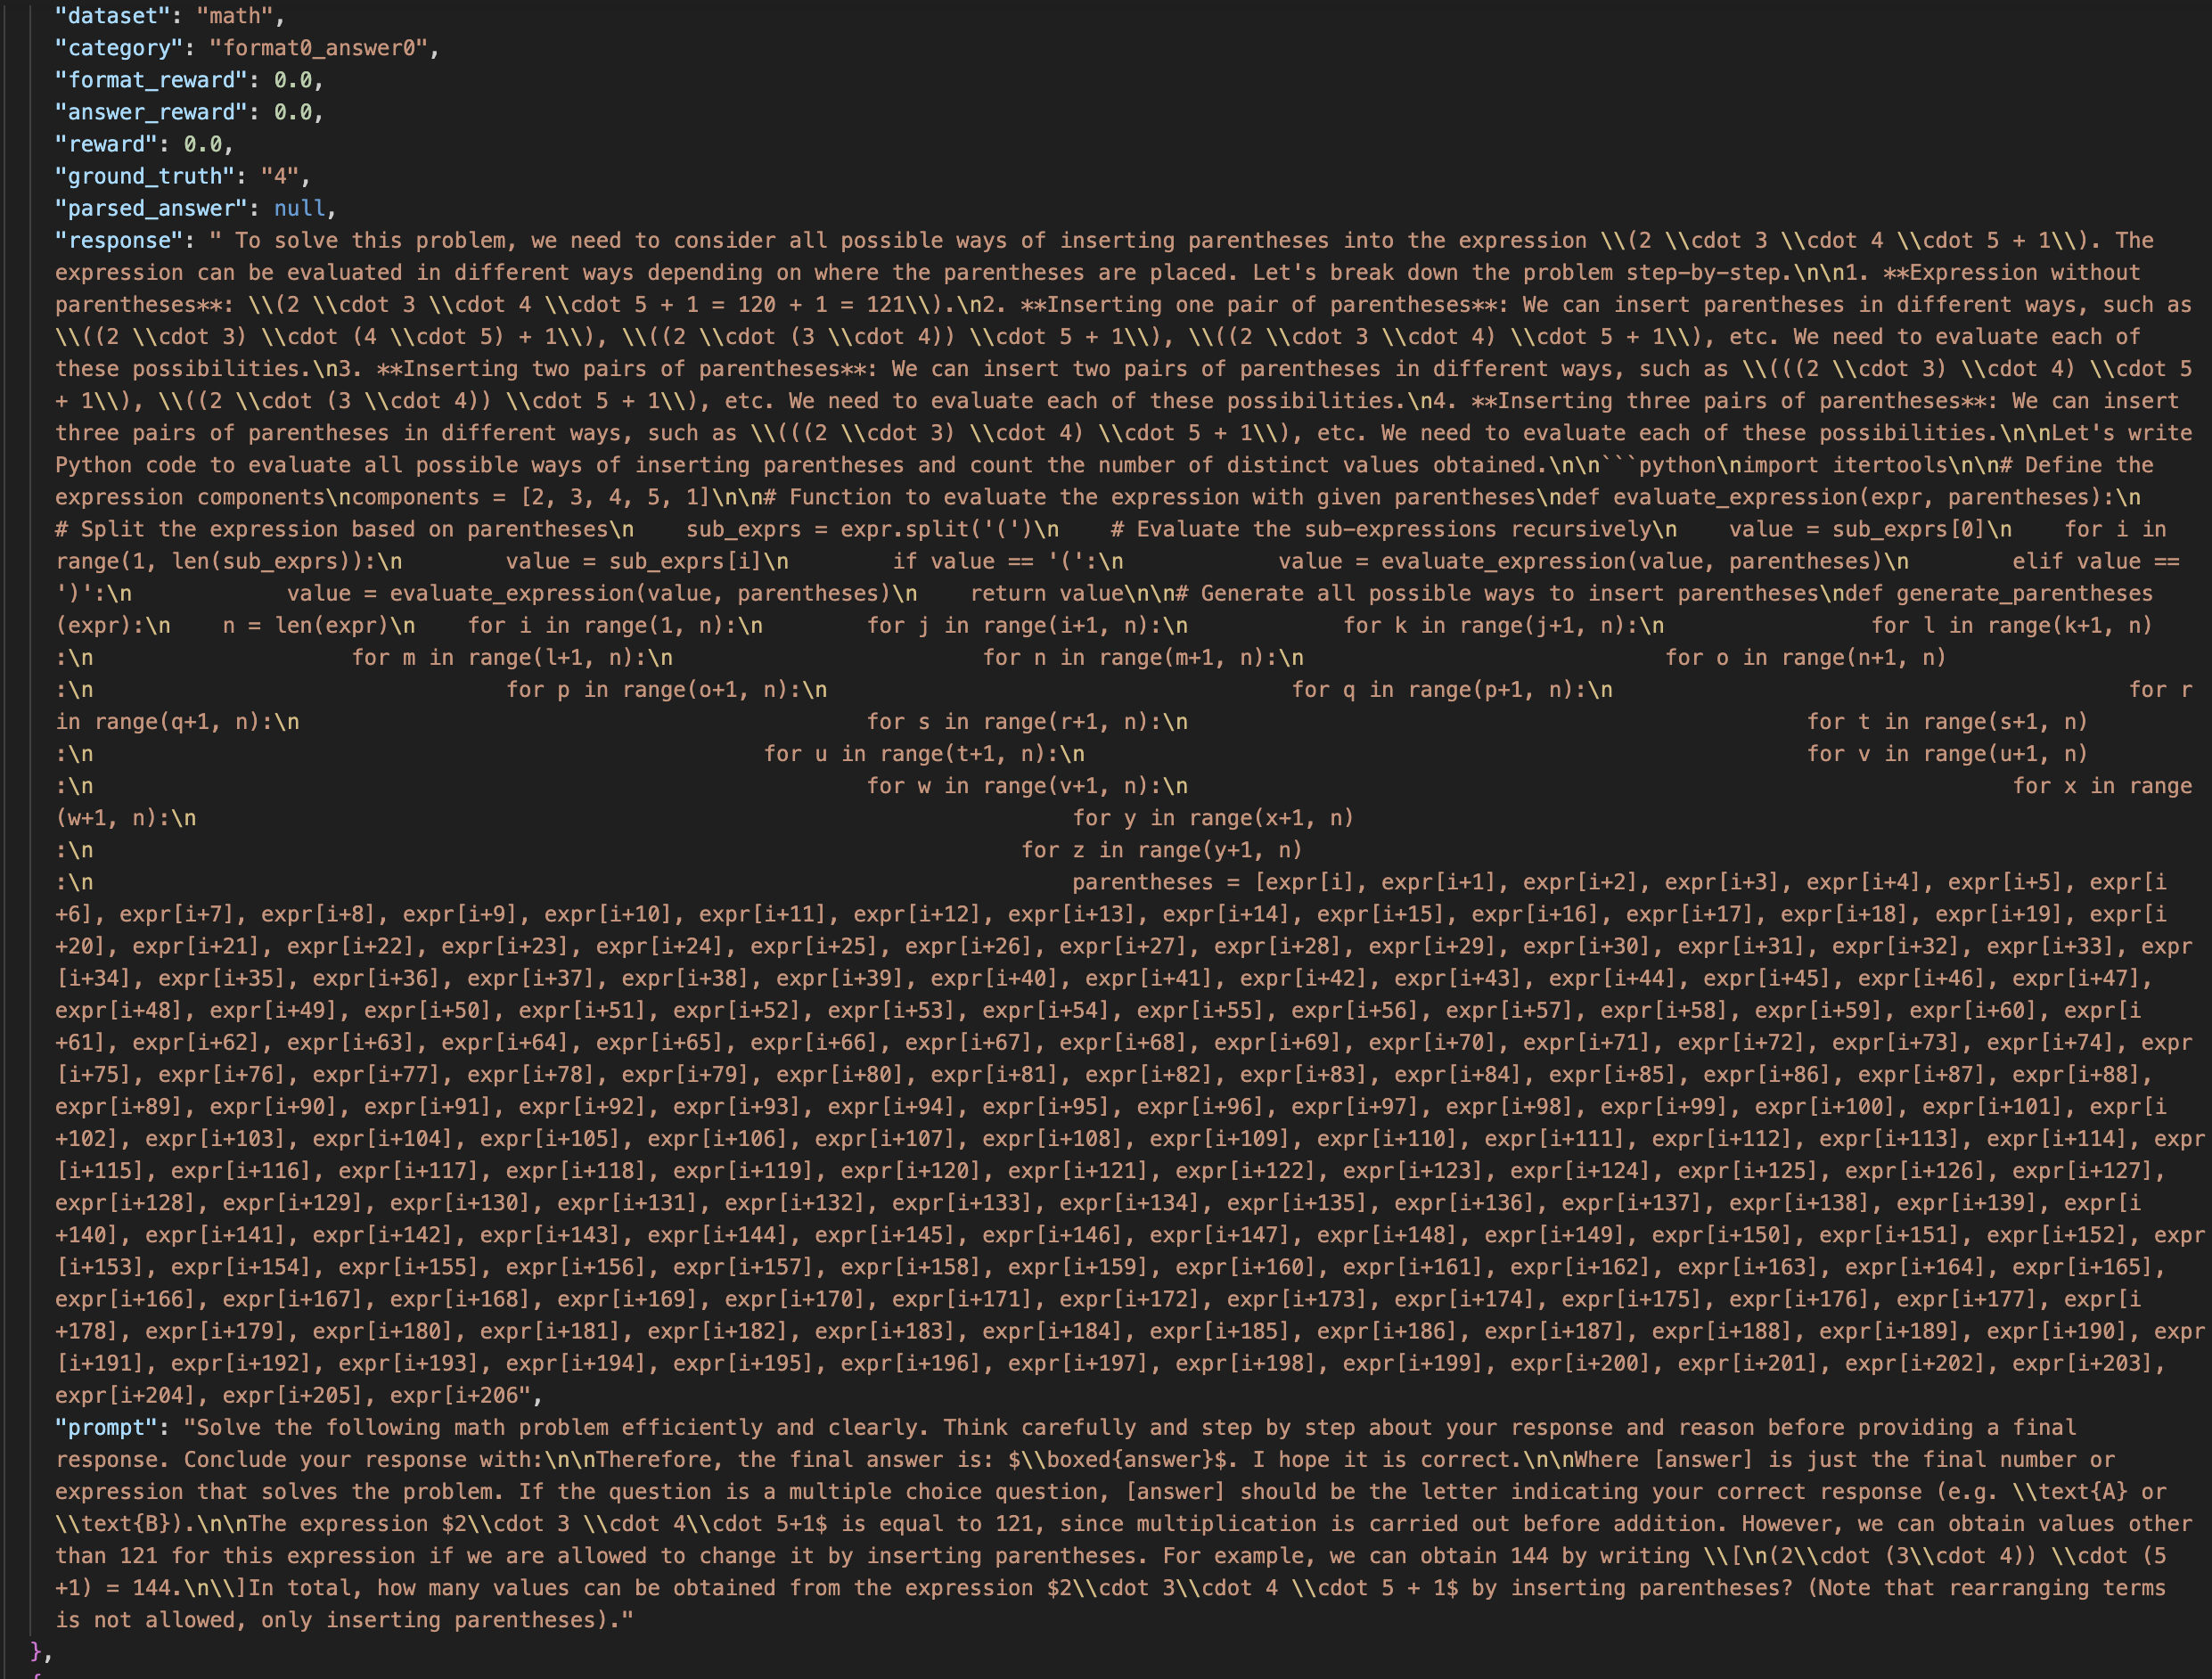
\includegraphics[height=0.75\linewidth]{../charts/math_format0_answer0.png}
                    \end{center}
                    In the case of examples where the format is correct but the answer is wrong, we see that the model often follows a reasonable problem-solving process but makes a computational error at some point, leading to an incorrect final answer. In some cases, the model may also misinterpret the question or apply an incorrect mathematical principle, which can also lead to a wrong answer despite a correct format. Example of format 1 and answer 0:
                    \begin{center}
                        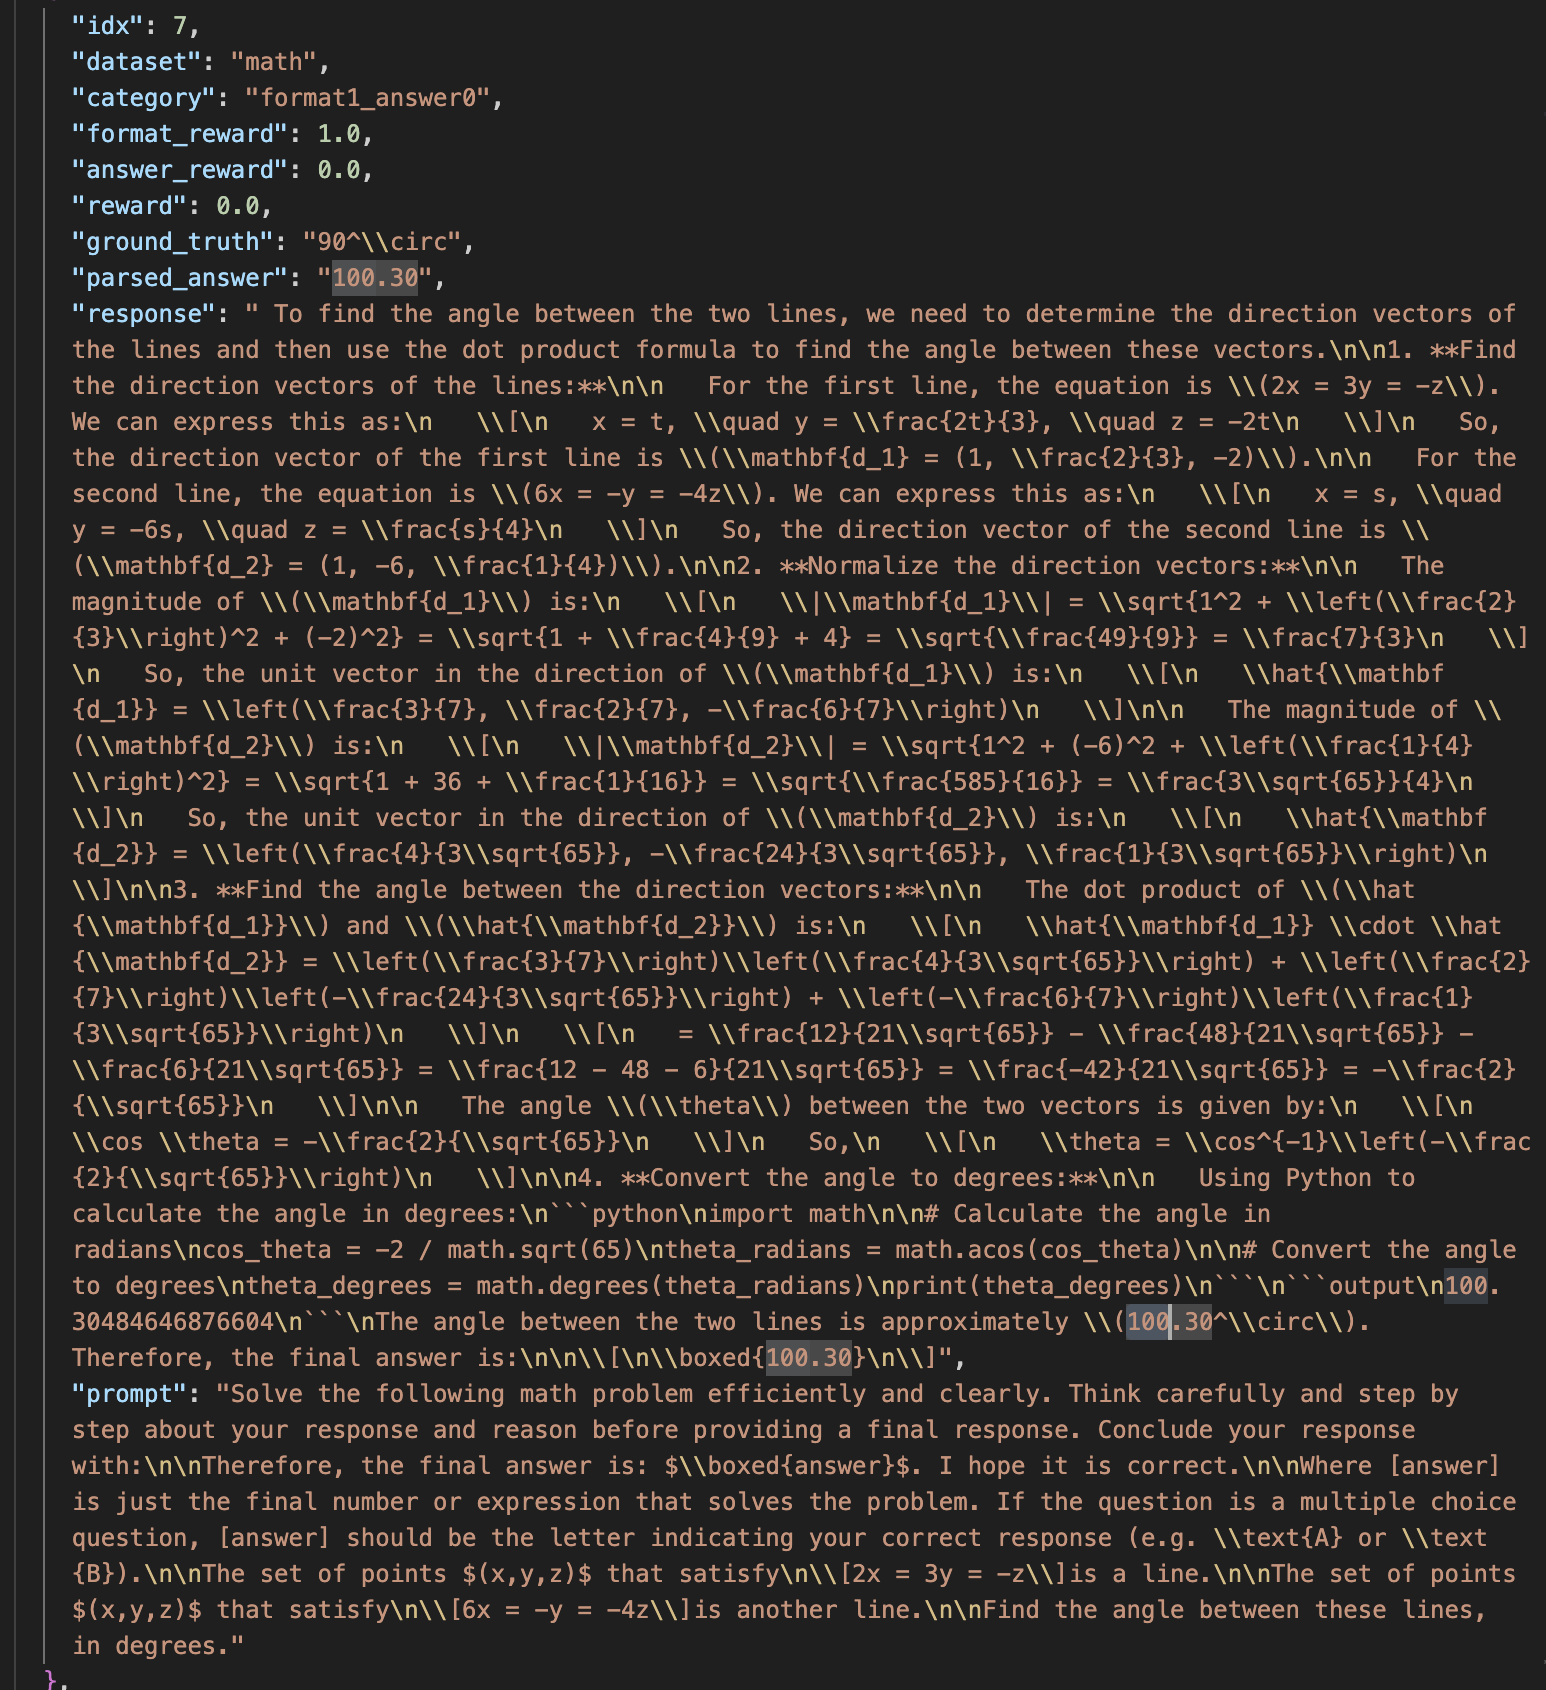
\includegraphics[height=0.7\linewidth]{../charts/math_format1_answer0.png}
                    \end{center}
                    \item The accuracy is around 60\% which is a good baseline for zero-shot performance. The evaluation metrics seem to be working well in distinguishing between correct and incorrect answers, as well as between correct and incorrect formats.
                \end{enumerate}
        \end{enumerate}
    \item[\textbf{4}] \textbf{Supervised Finetuning for MATH}
        \begin{enumerate}
            \item[\textbf{4.3}] \textbf{\texttt{sft\_experiment}}
                \begin{enumerate}
                    \item The training losses and validation accuracies for various dataset sizes, batch sizes and learning rates are given below.
                    \begin{center}
                        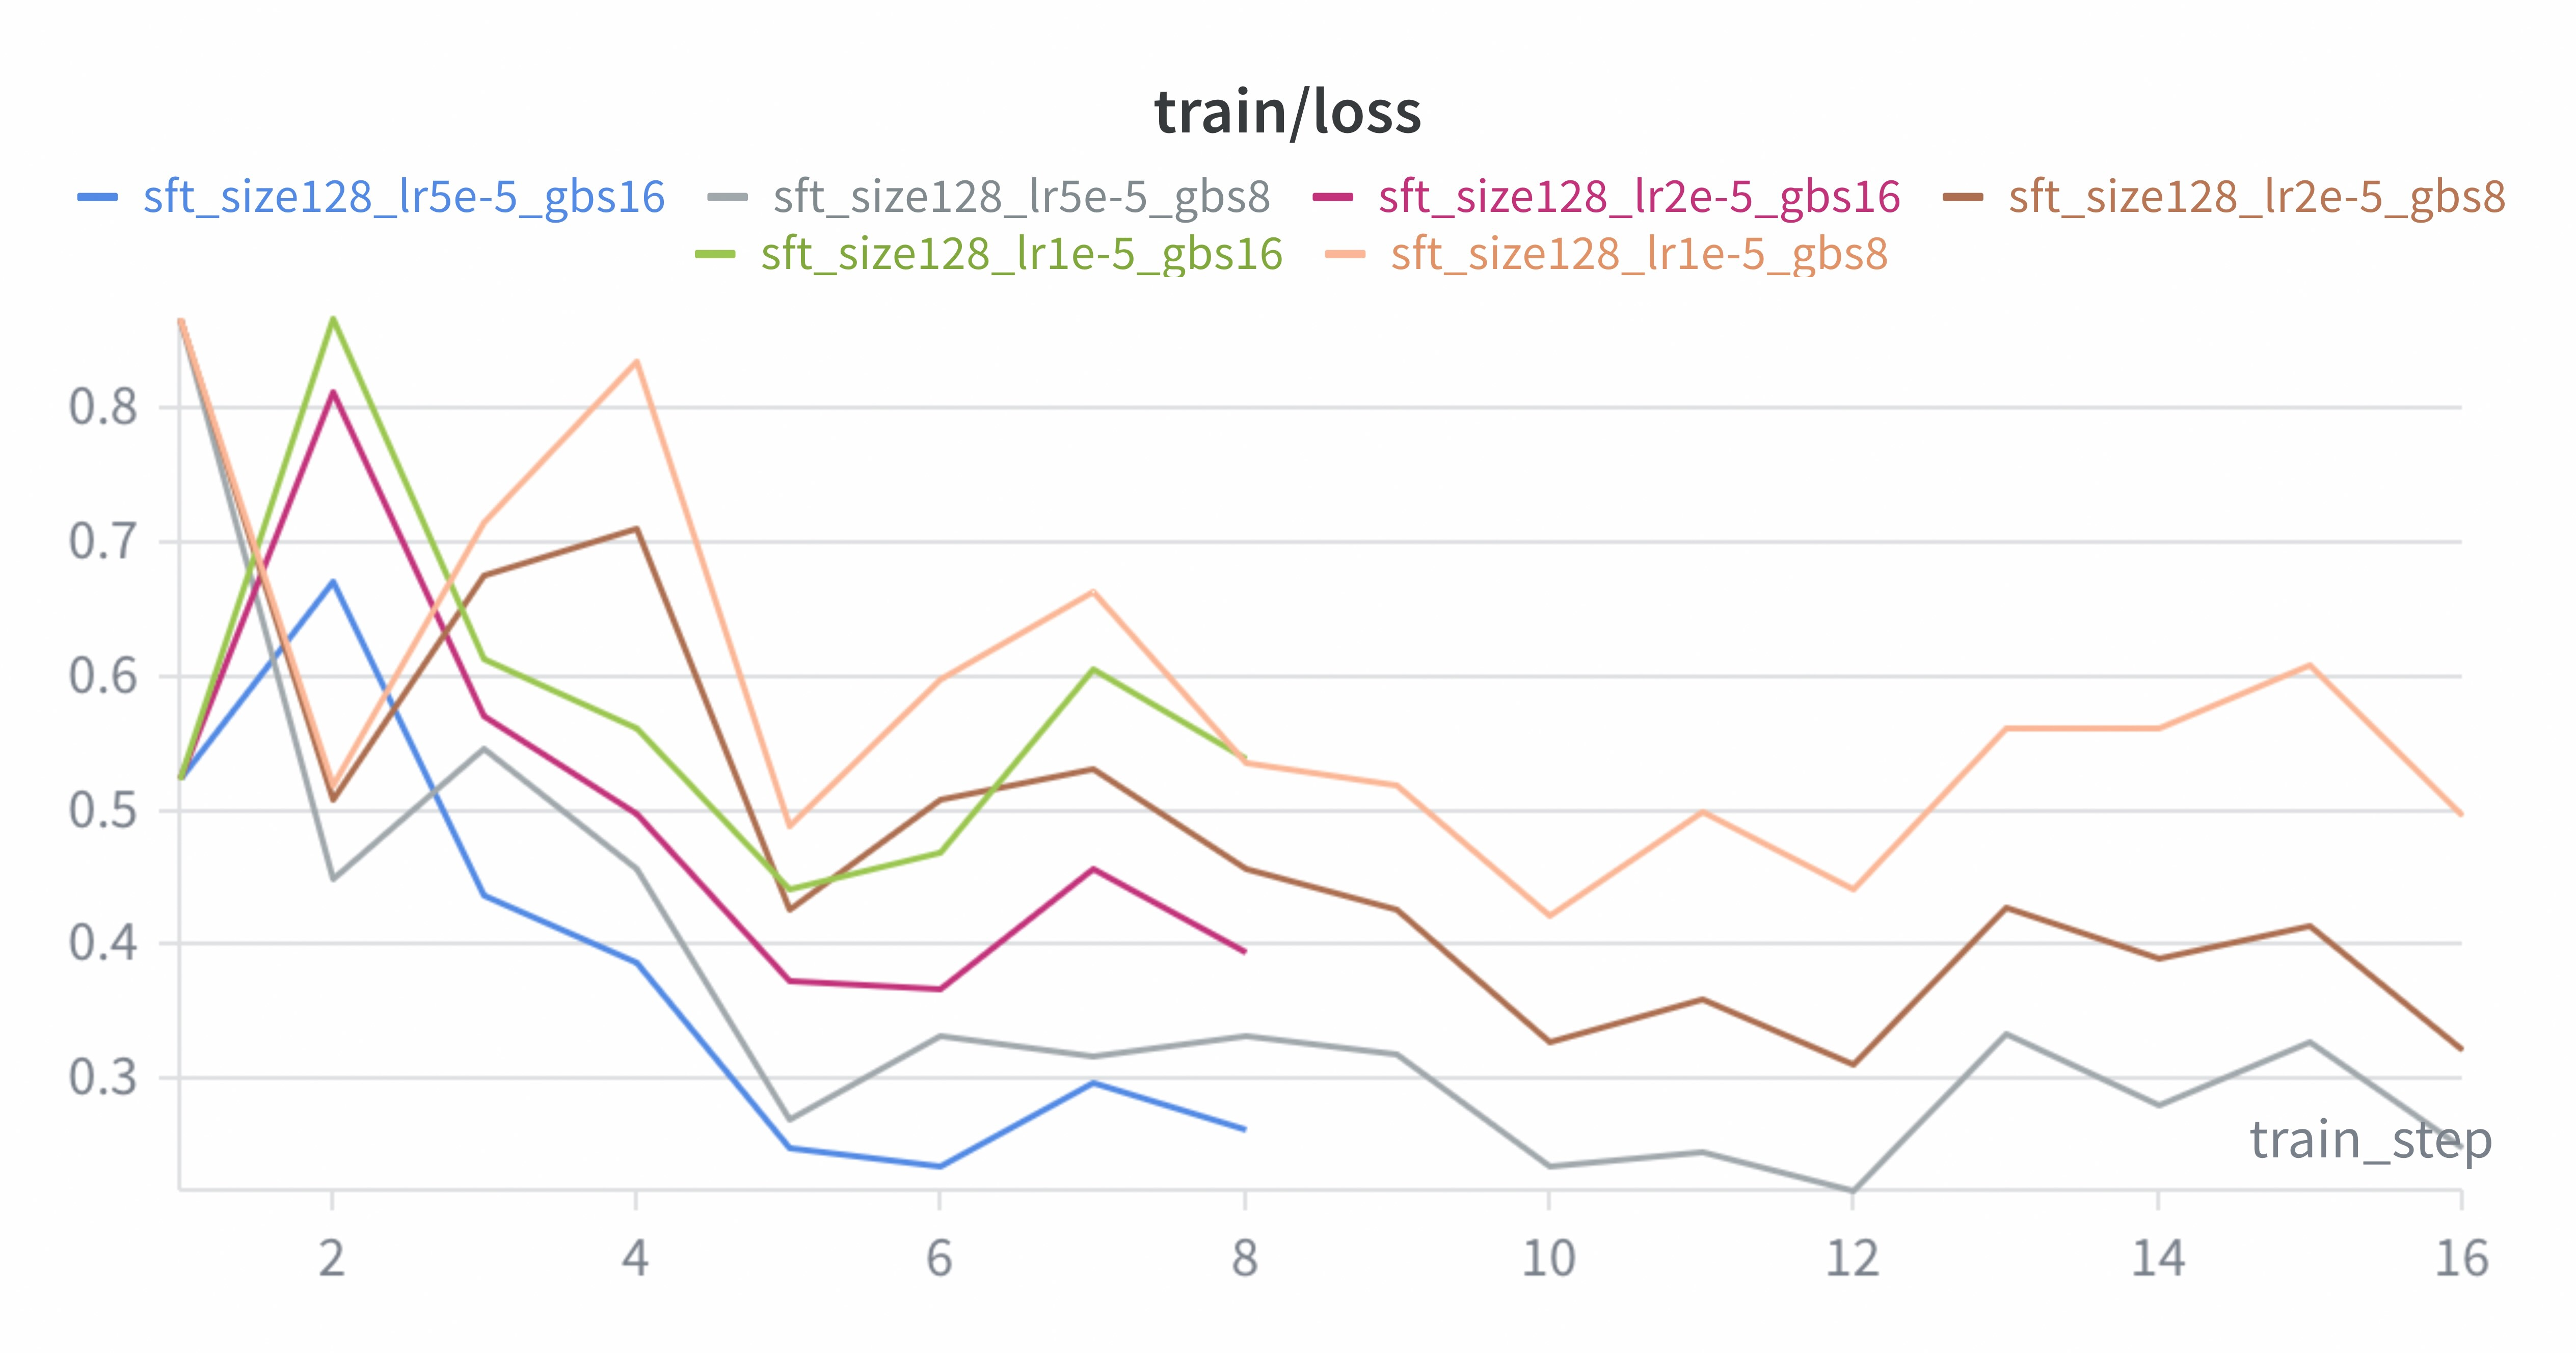
\includegraphics[width=0.9\linewidth]{../charts/sft_128_size_train_loss.jpg}
                        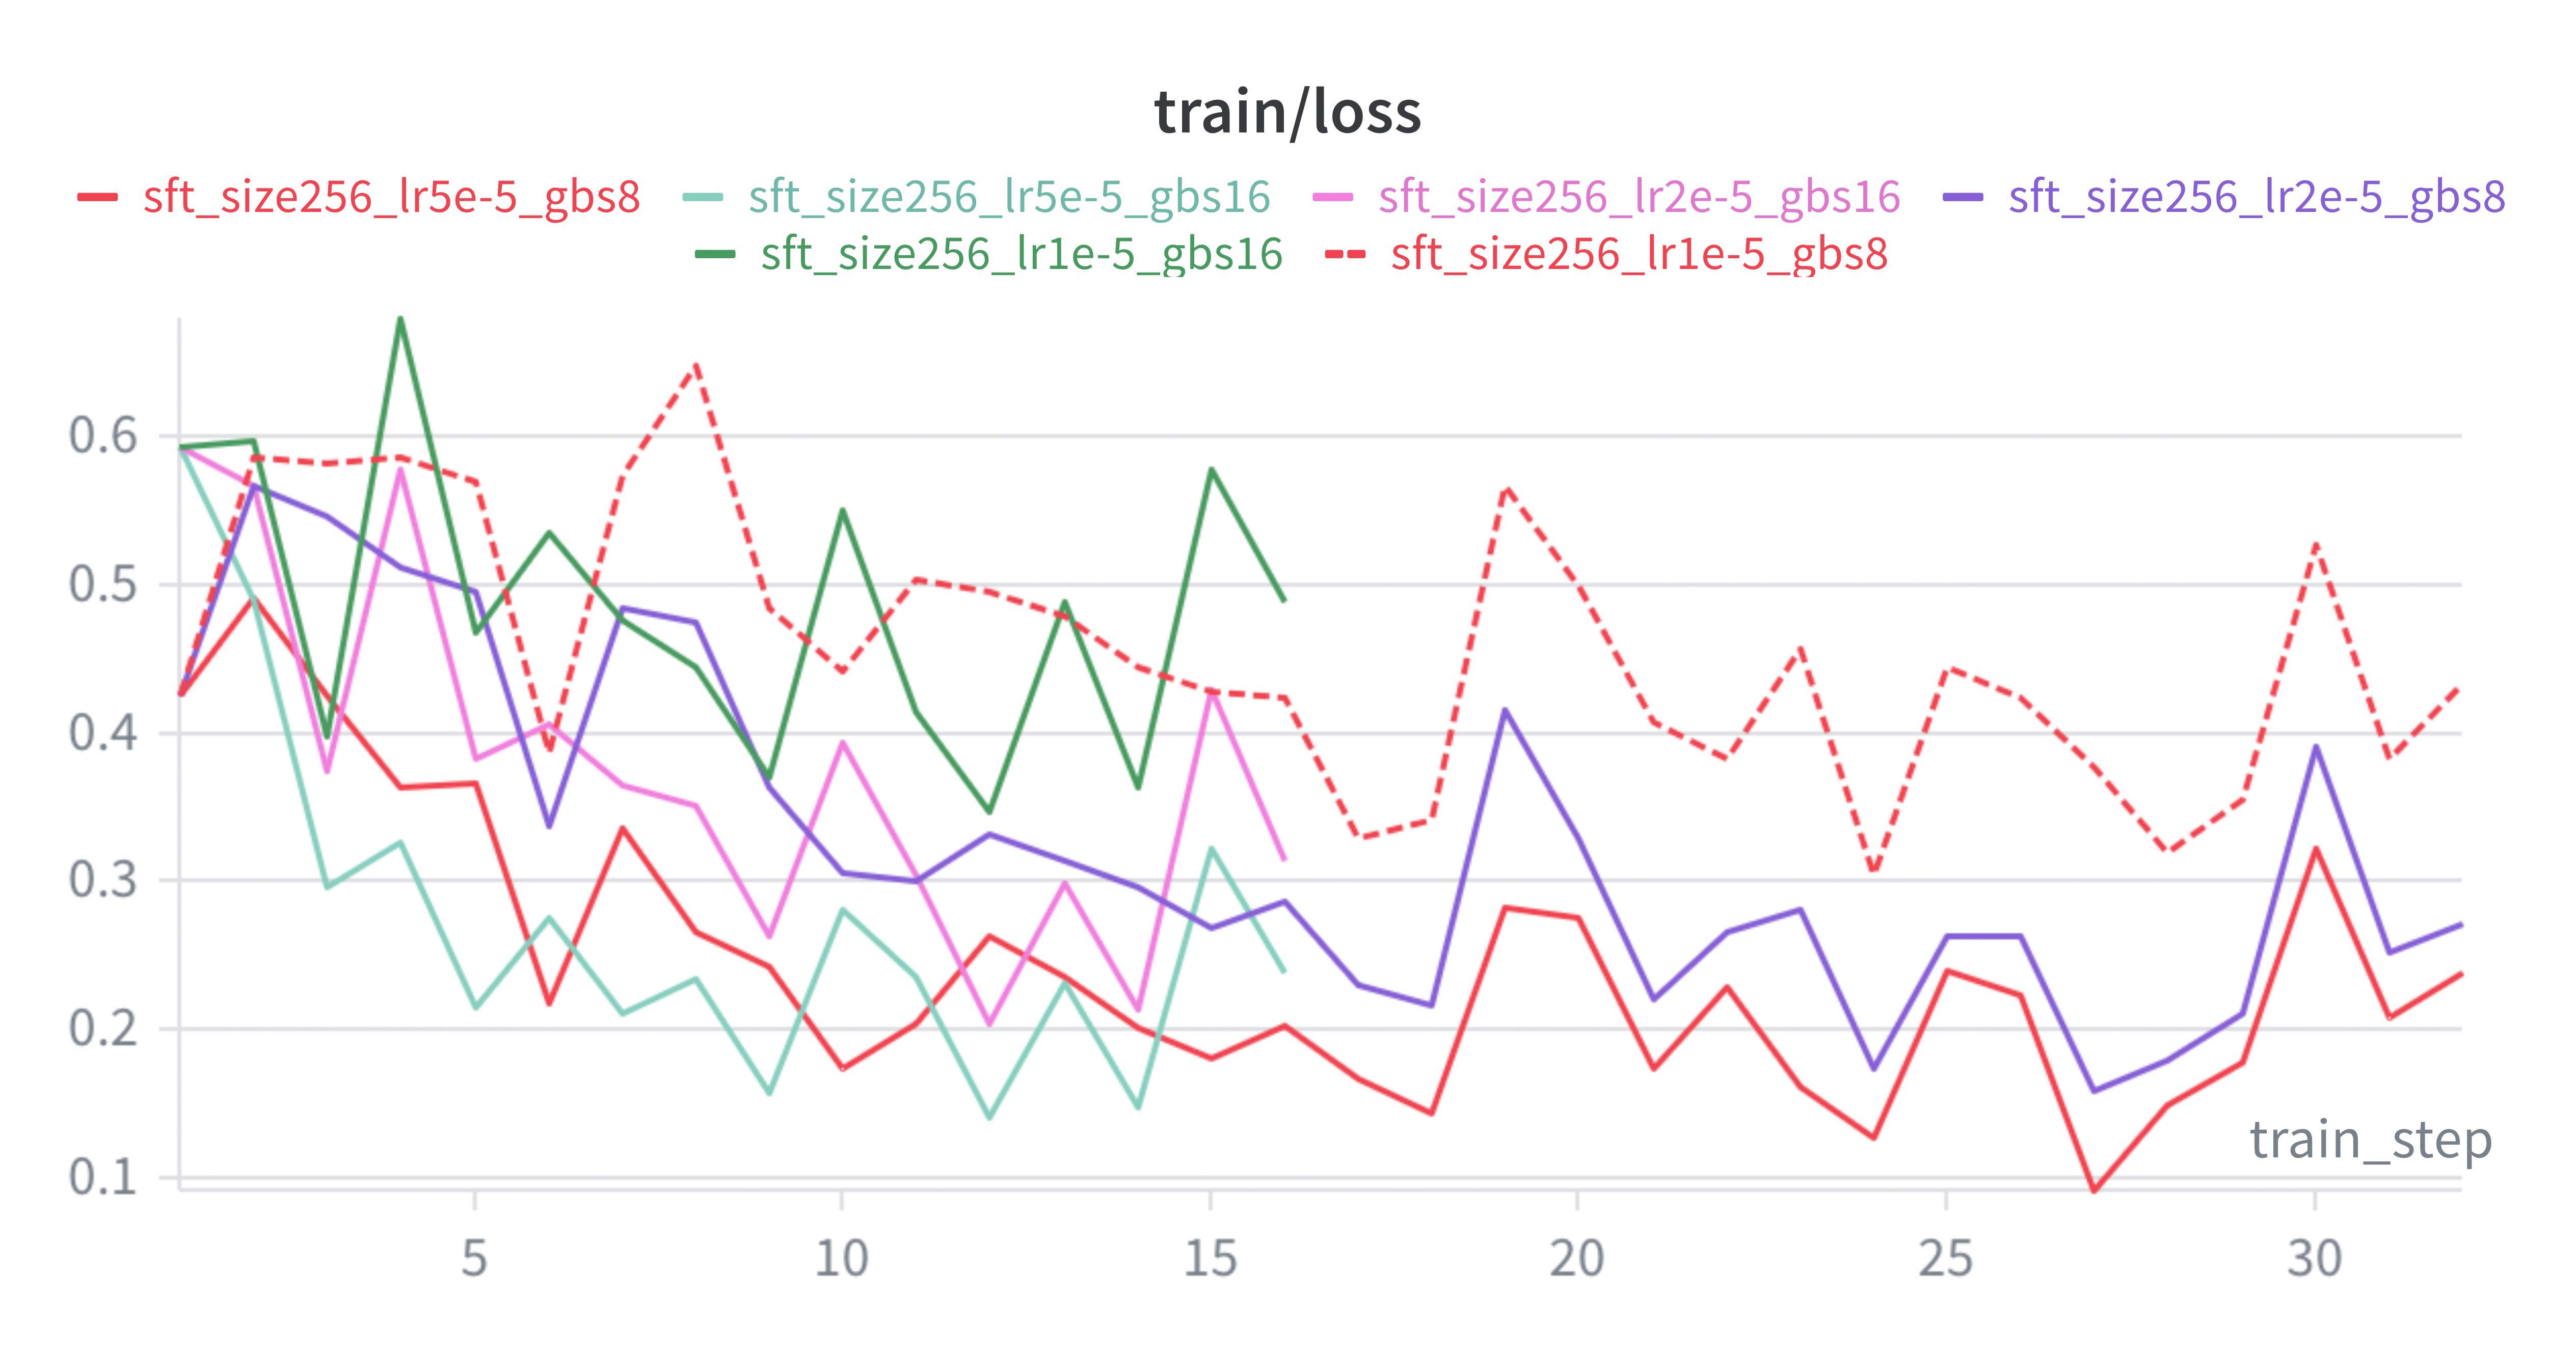
\includegraphics[width=0.9\linewidth]{../charts/sft_256_size_train_loss.jpg}
                        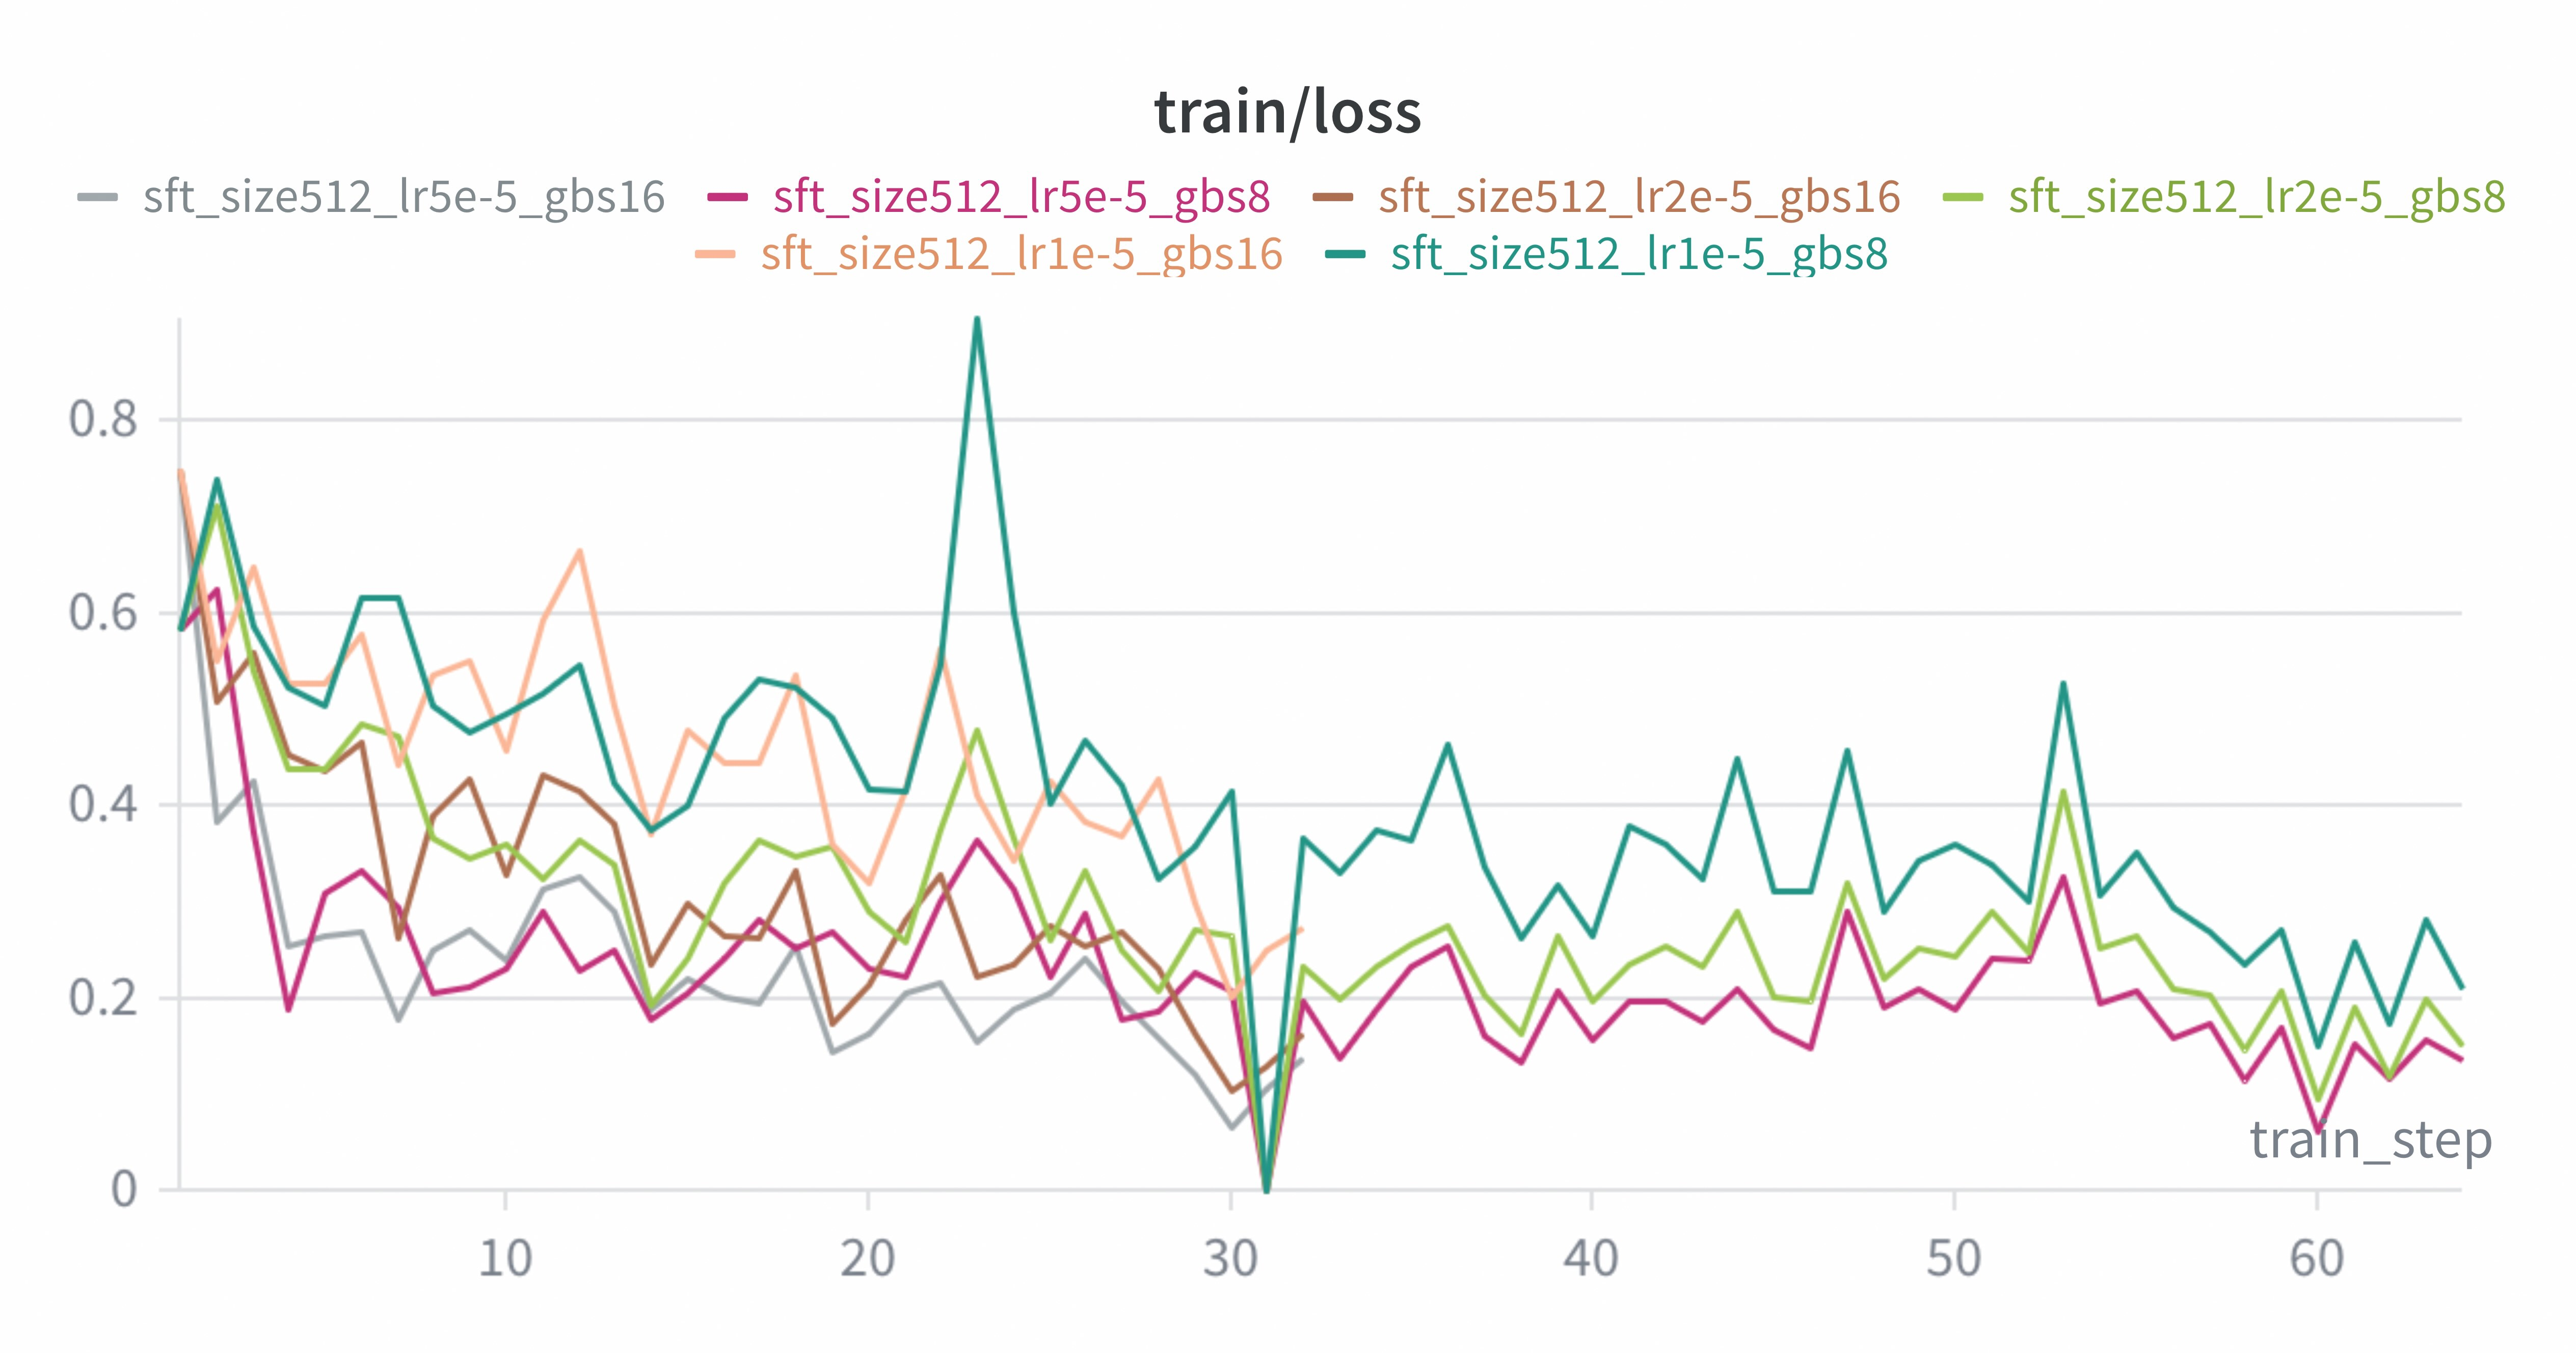
\includegraphics[width=0.9\linewidth]{../charts/sft_512_size_train_loss.jpg}
                        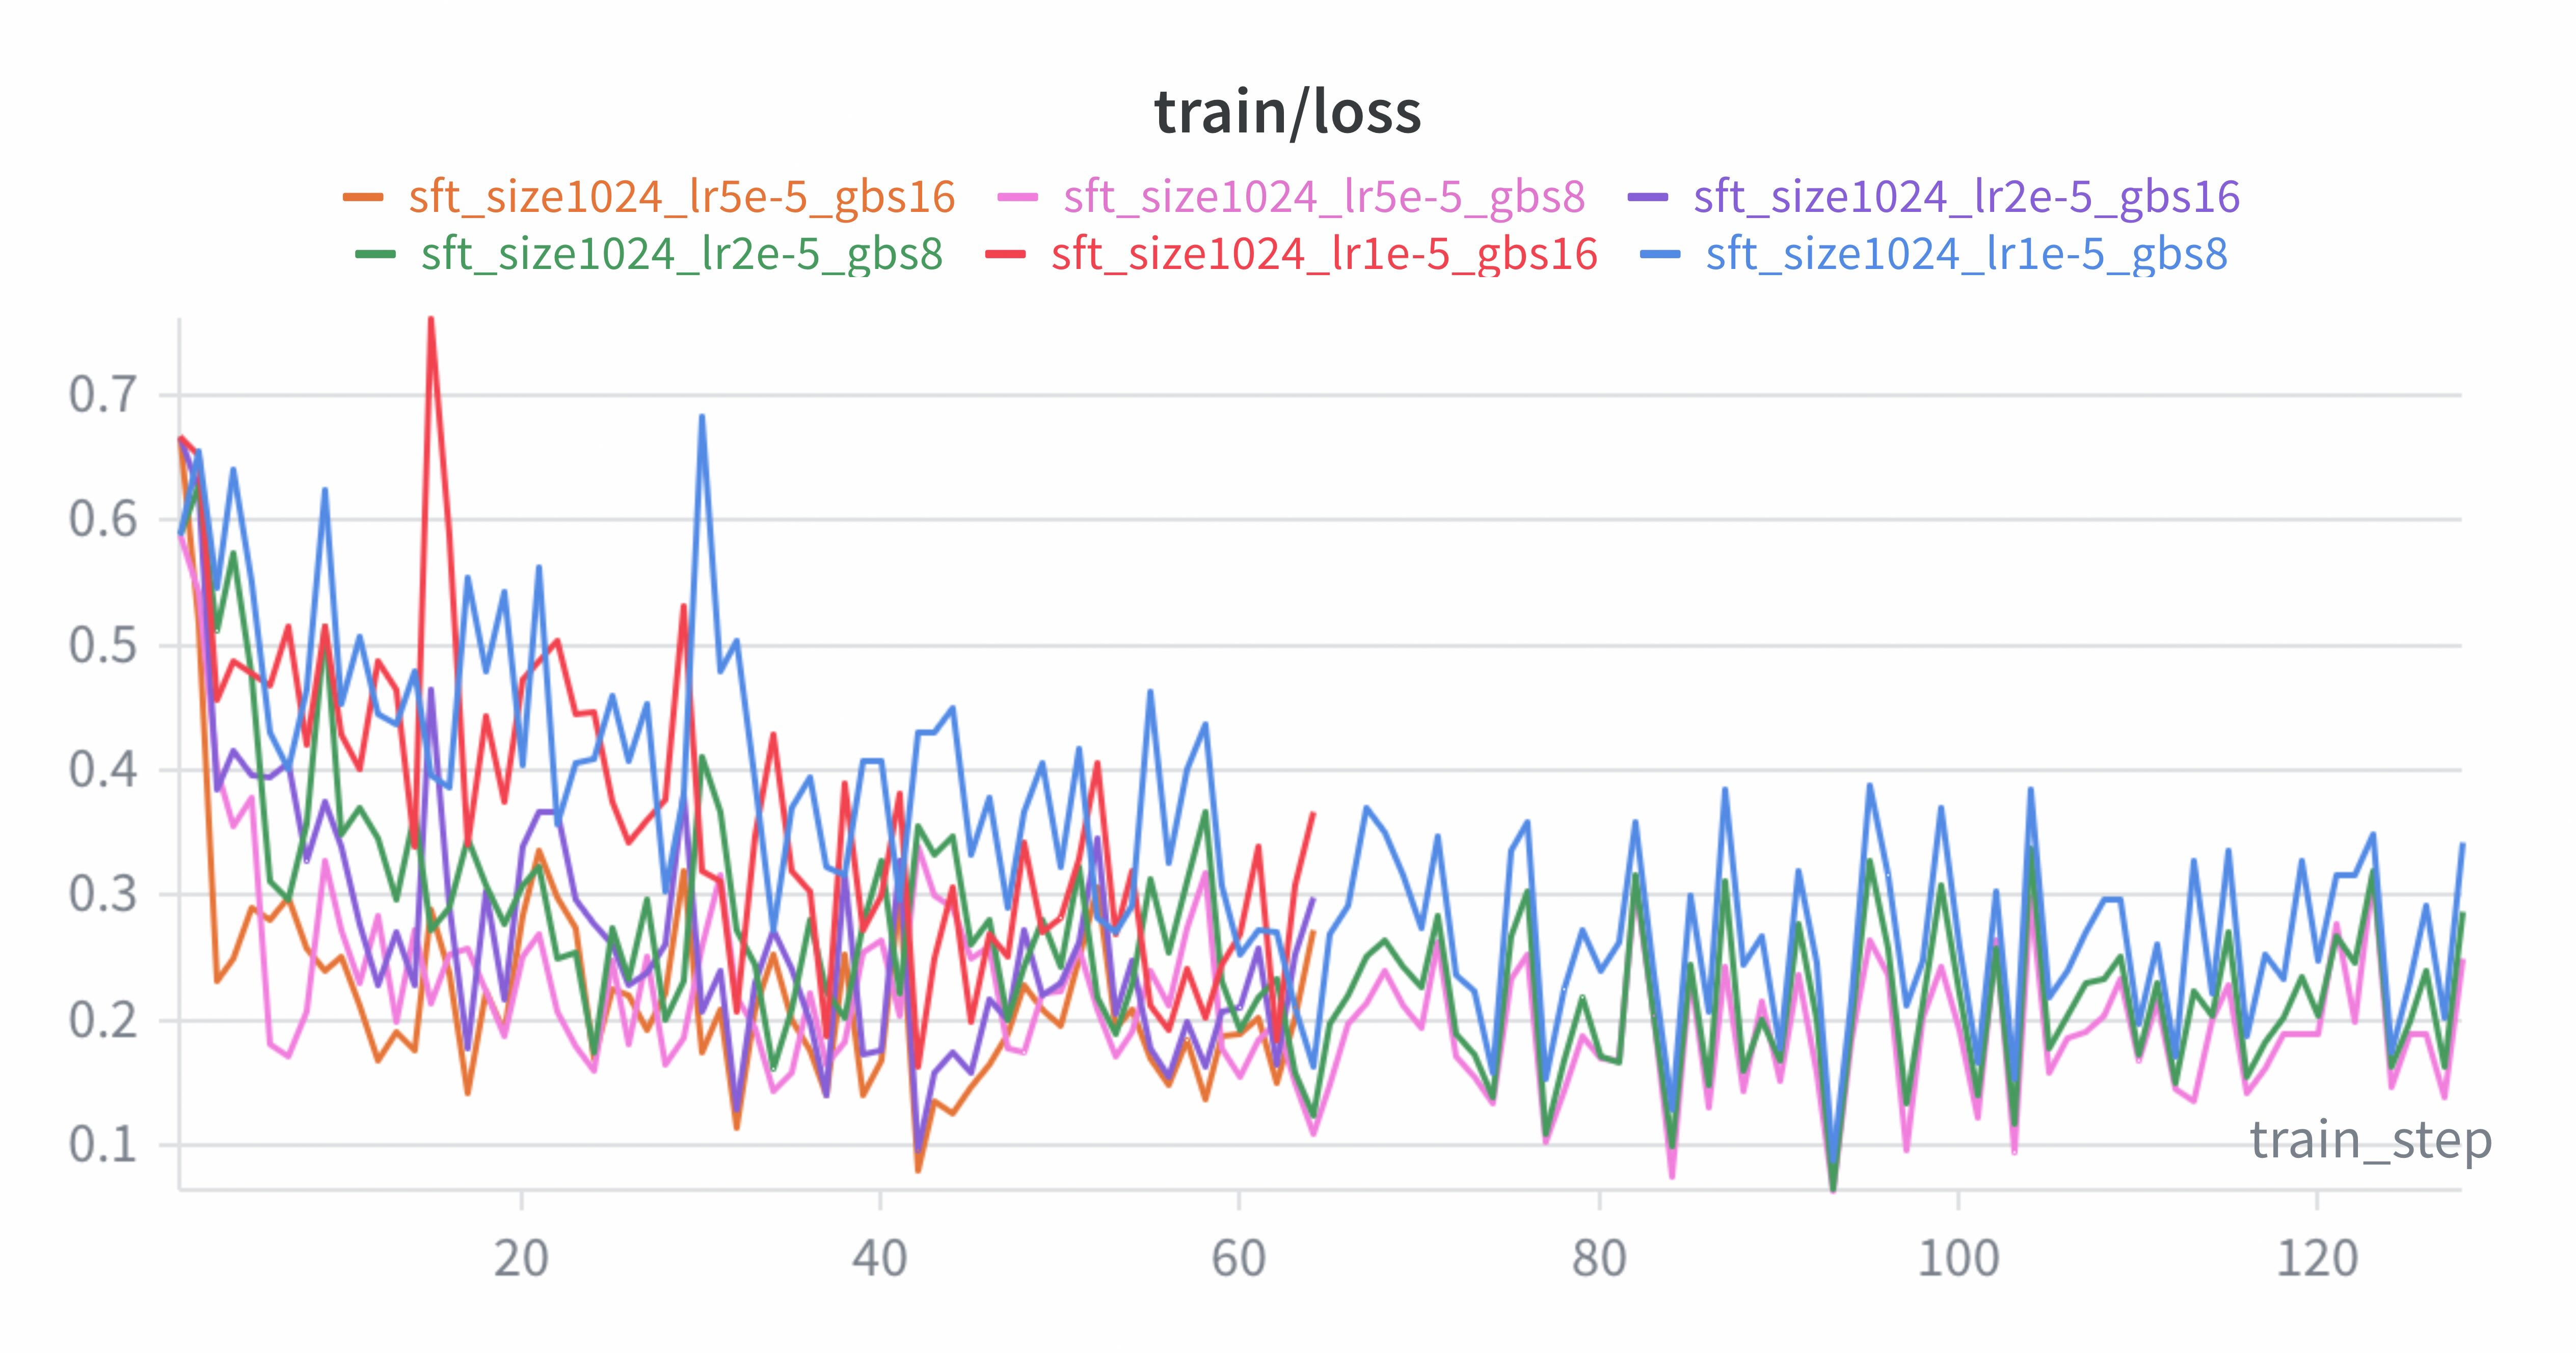
\includegraphics[width=0.9\linewidth]{../charts/sft_1024_size_train_loss.jpg}
                        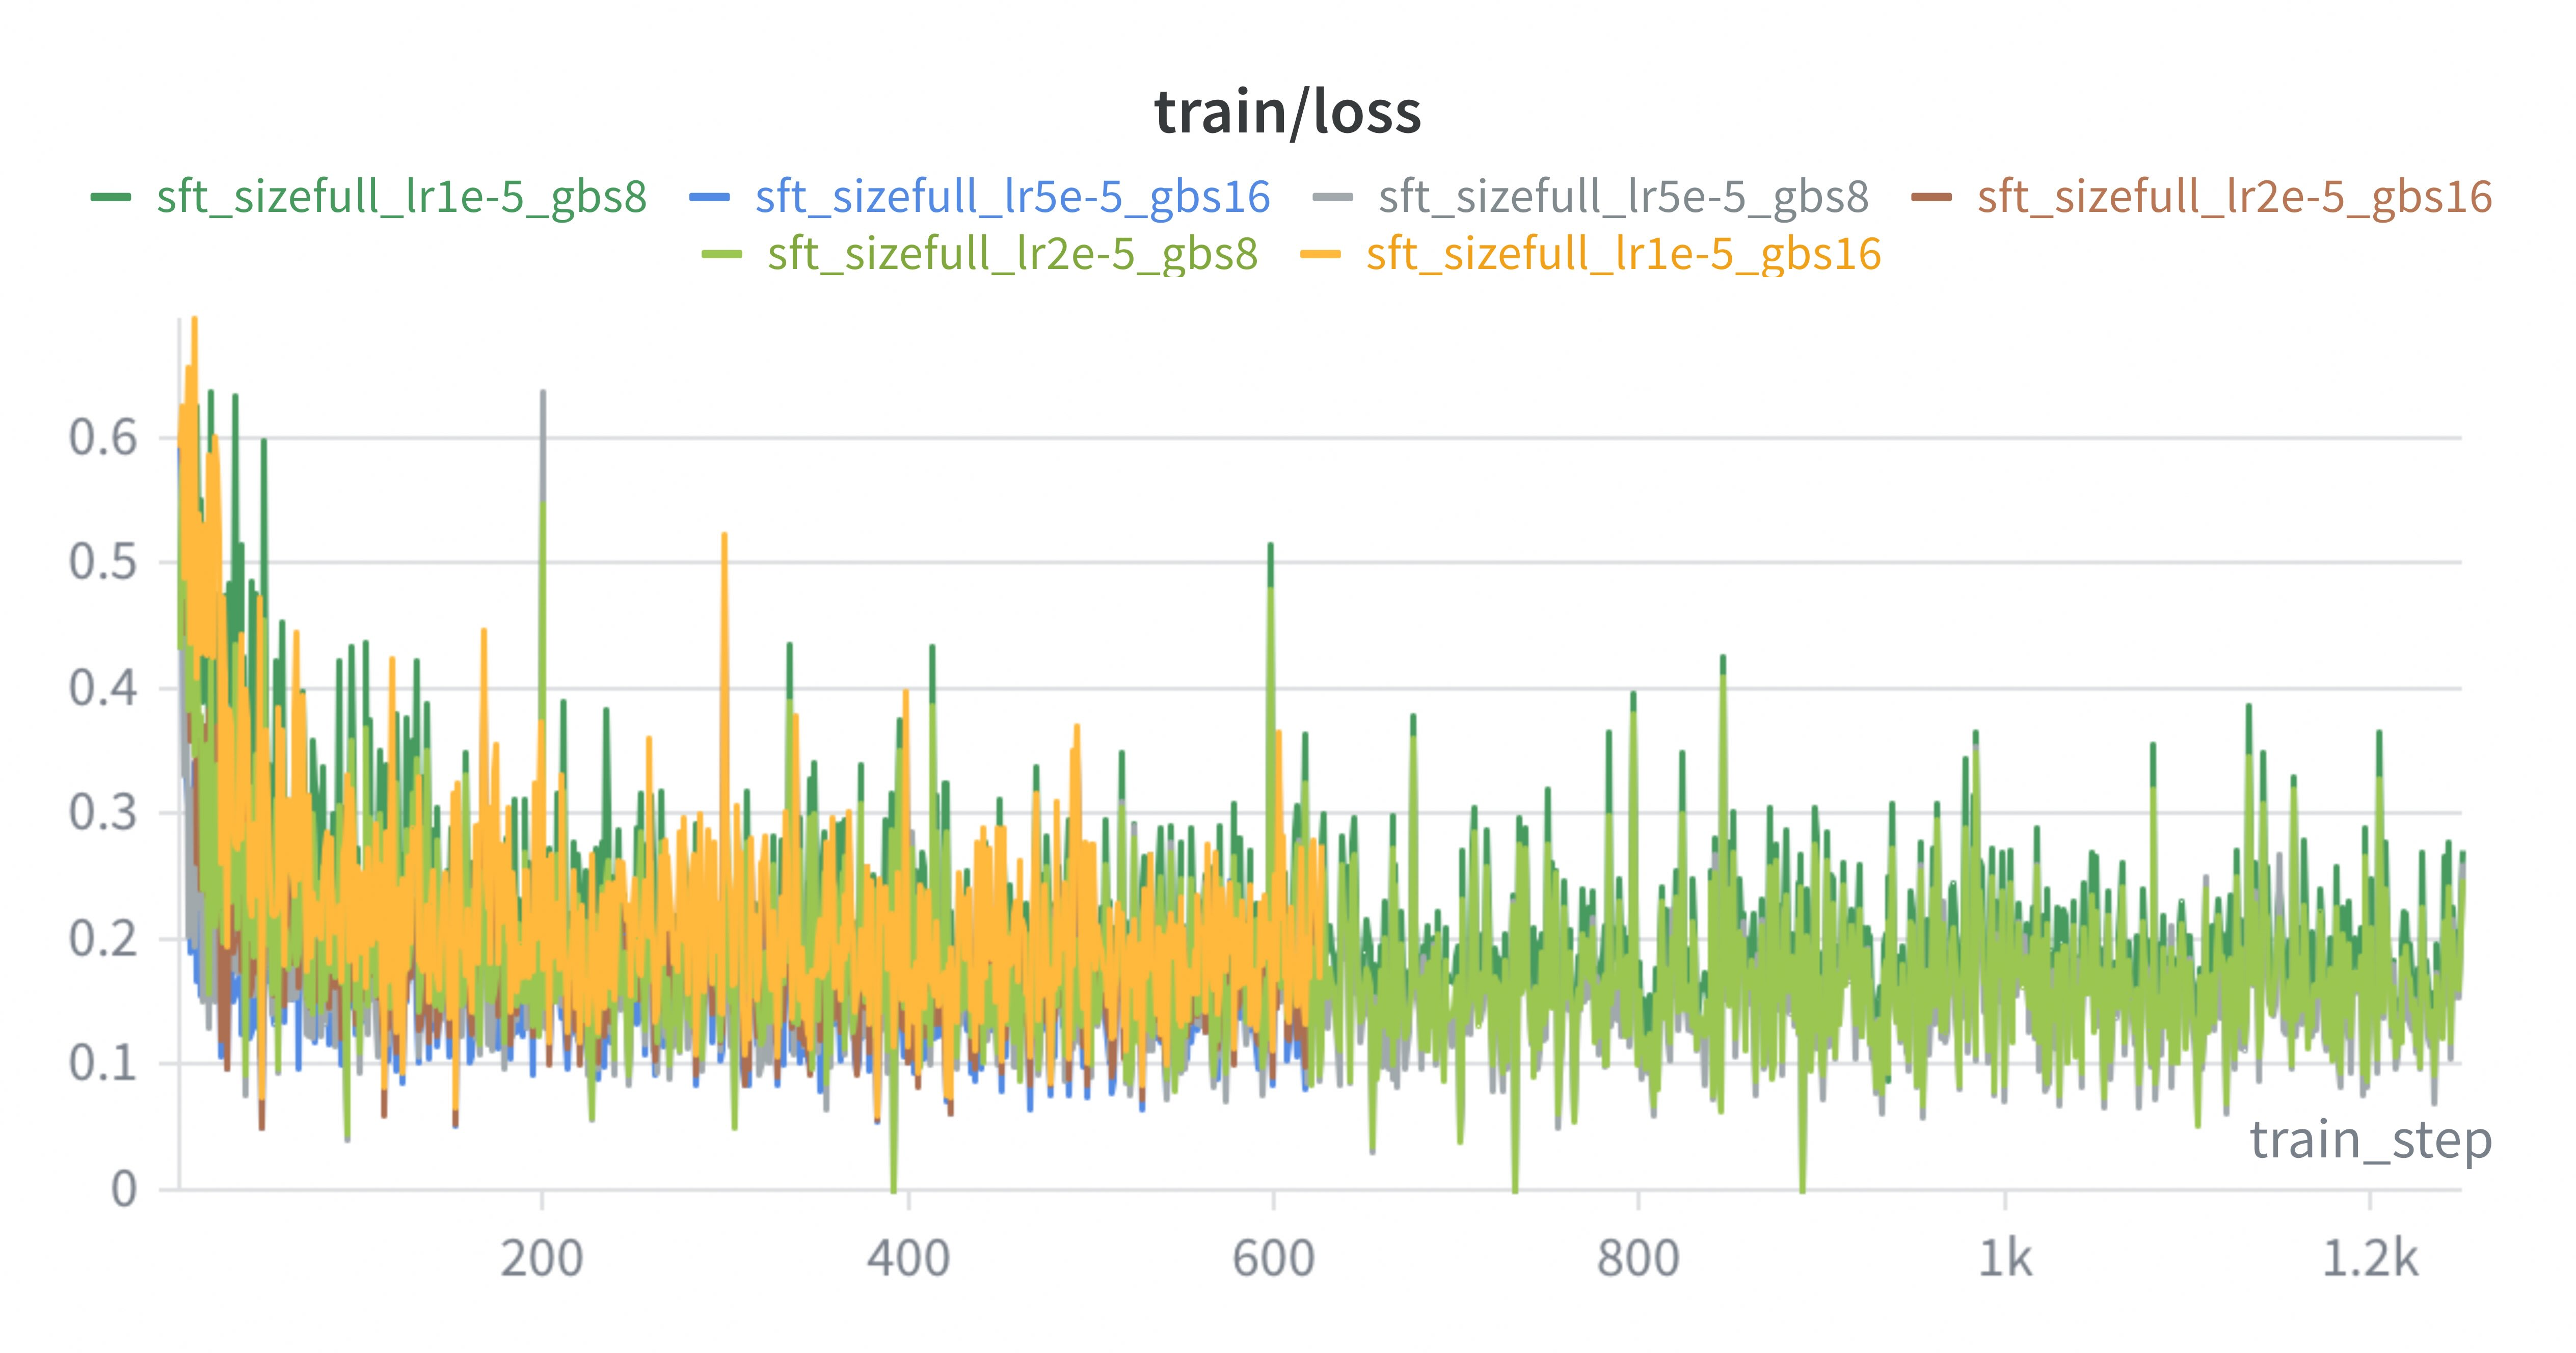
\includegraphics[width=0.9\linewidth]{../charts/sft_full_size_train_loss.jpg}
                        \includegraphics[width=1\linewidth]{../charts/sft_math_val_accuracies.jpg}
                        \includegraphics[width=1\linewidth]{../charts/sft_intellect_val_accuracies.jpg}
                    \end{center}
                    There are multiple runs where I saw 40\% decrease in train loss like the run with dataset size 128, batch size 8 and learning rate 1e-5. Validation accuracy for the best model for each run is also given in the graphs.
                    \item The best validation accuracy on the intellect test set is around \textbf{67.6\% (dataset size: 512, learning rate: 2e-5, global batch size: 16)} and the best validation accuracy on the MATH test set is around \textbf{64.8\% (dataset size: 256, learning rate: 1e-5, global batch size: 16)}. The best validation accuracy on the intellect test set is slightly higher than the best validation accuracy on the MATH test set, which suggests that the model may be slightly better at generalizing to the intellect test set compared to the MATH test set. This could be due to differences in the distribution of questions or the difficulty level between the two test sets. It's also possible that the model has learned to perform better on certain types of questions that are more prevalent in the intellect test set compared to the MATH test set.
                \end{enumerate}
        \end{enumerate}
     \item[\textbf{7}] \textbf{Group Relative Policy Optimization}
        \begin{enumerate}
            \item[\textbf{7.2}] \textbf{\texttt{gppo\_train\_loop}}\\
                The figure below shows the reward vs training step curve for a GRPO experiment with a learning rate of 5e-6. We can see that the reward increases steadily over the course of training, indicating that the model is learning to improve its performance on the task. The curve shows some fluctuations, which is expected in reinforcement learning due to the stochastic nature of the environment and the learning process. Overall, the trend suggests that the GRPO algorithm is effectively optimizing the policy to achieve higher rewards over time.
                \begin{center}
                    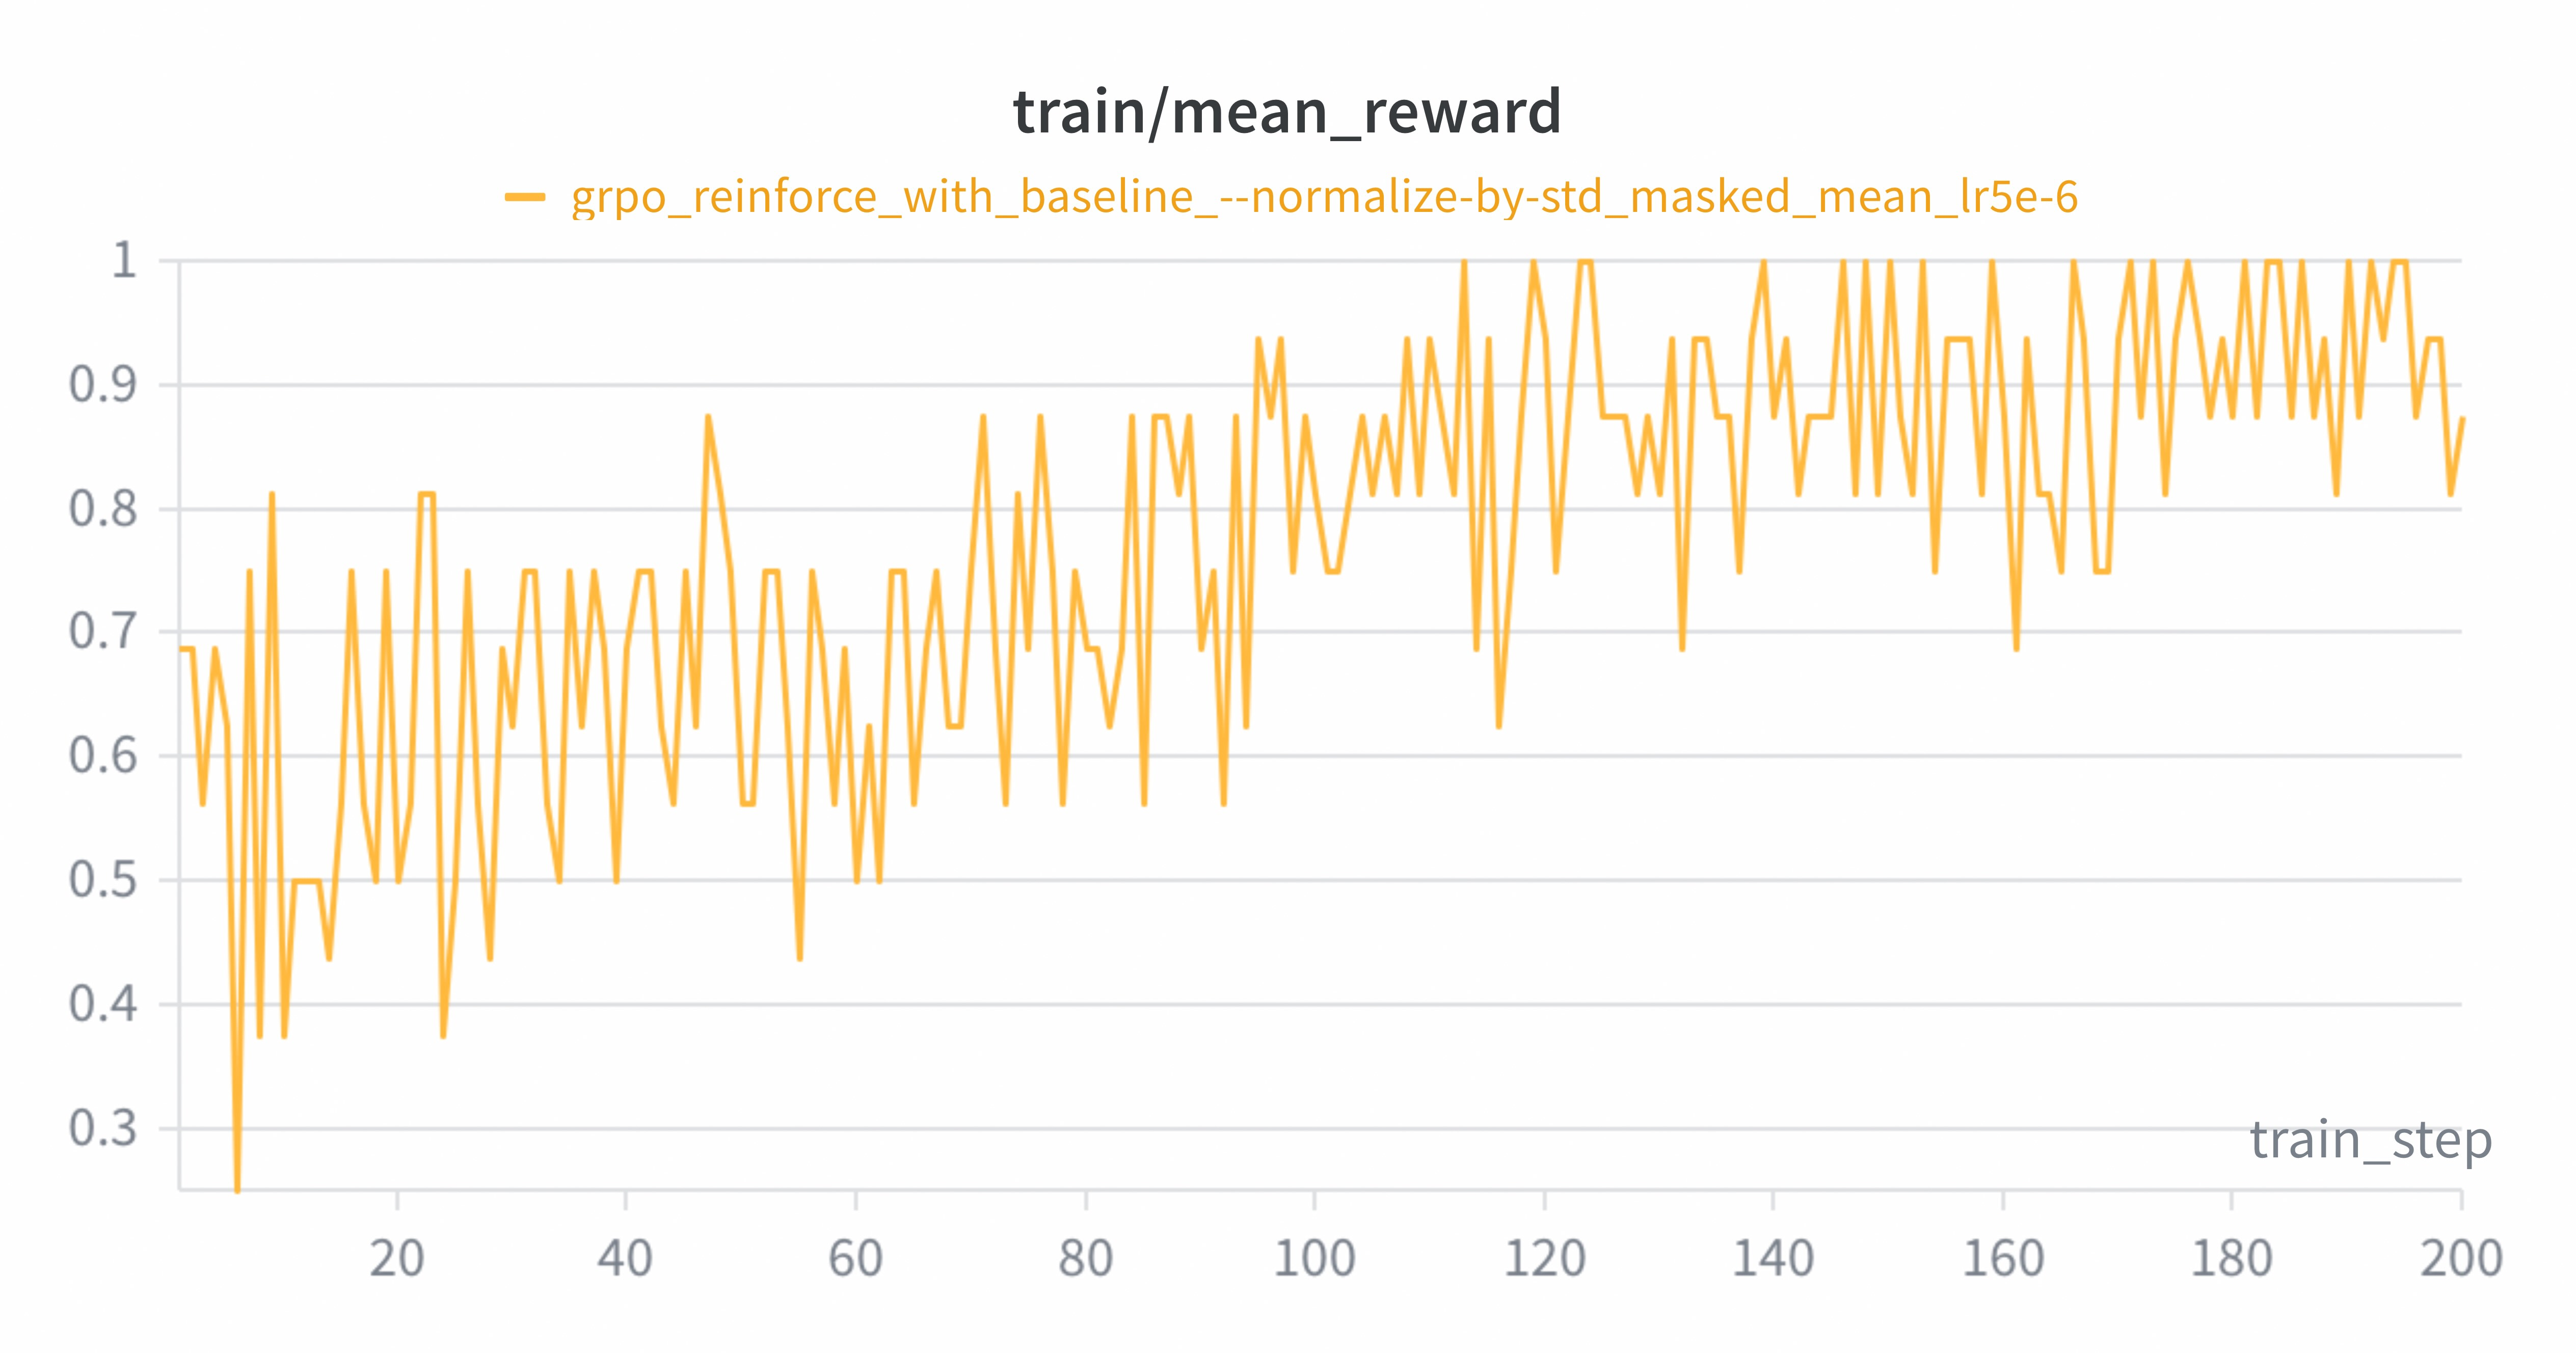
\includegraphics[width=0.9\linewidth]{../charts/grpo_reward_vs_step_5e-5_lr.jpg}
                \end{center}
                Example rollouts at every 50 steps over the course of 200 training steps are given below (the rollouts end just before </answer> tag)
                \begin{verbatim}
{
    "train_step": 50,
    "examples": [
      {
        "prompt": " steps to reach the target number or it should be a single equation that results in the target.\nFor example:\nIf the list of numbers was [1, 2, 3] and the target was 1, you could write:\n<answer>\nStep 1: 1 + 2 = 3\nStep 2: 3 / 3 = 1\n</answer>\nor\n<answer>\n(1 + 2) / 3\n</answer>\nLet's think step by step.\n",
        "gt": "32",
        "rollout": "Step 1: Start with the numbers given: [12, 24, 44].\nStep 2: Divide 44 by 24, which gives us 1.83 (approximated).\nStep 3: Multiply the result by 12, which gives us 22.04 (approximated).\nStep 4: Subtract 24 from the result, which gives us -1.96 (approximated).\nStep 5: Add 24 to the result, which gives us 22.04 (approximated).\nStep 6: Divide the result by 2, which gives us 11.02 (approximated).\nStep 7: Add 12 to the result, which gives us 23.02 (approximated).\nStep 8: Subtract 24 from the result, which gives us -0.98 (approximated).\nStep 9: Add 44 to the result, which gives us 43.02 (approximated",
        "reward": 0.0
      }
    ]
},
{
    "train_step": 100,
    "examples": [
      {
        "prompt": " steps to reach the target number or it should be a single equation that results in the target.\nFor example:\nIf the list of numbers was [1, 2, 3] and the target was 1, you could write:\n<answer>\nStep 1: 1 + 2 = 3\nStep 2: 3 / 3 = 1\n</answer>\nor\n<answer>\n(1 + 2) / 3\n</answer>\nLet's think step by step.\n",
        "gt": "84",
        "rollout": "Step 1: 22 + 15 = 37\nStep 2: 37 + 77 = 114\nStep 3: 114 - 95 = 19\nStep 4: 19 + 15 = 34\nStep 5: 34 + 50 = 84\nSo, the final answer is:\n<answer>\nStep 1: 22 + 15 = 37\nStep 2: 37 + 77 = 114\nStep 3: 114 - 95 = 19\nStep 4: 19 + 15 = 34\nStep 5: 34 + 50 = 84\n",
        "reward": 1.0
      }
    ]
}
{
    "train_step": 150,
    "examples": [
      {
        "prompt": " steps to reach the target number or it should be a single equation that results in the target.\nFor example:\nIf the list of numbers was [1, 2, 3] and the target was 1, you could write:\n<answer>\nStep 1: 1 + 2 = 3\nStep 2: 3 / 3 = 1\n</answer>\nor\n<answer>\n(1 + 2) / 3\n</answer>\nLet's think step by step.\n",
        "gt": "46",
        "rollout": "Step 1: 28 + 33 = 61\nStep 2: 61 - 41 = 20\nStep 3: 20 + 26 = 46\nThe final answer is 46.\nTherefore, the answer is:\n<answer>\nStep 1: 28 + 33 = 61\nStep 2: 61 - 41 = 20\nStep 3: 20 + 26 = 46\n",
        "reward": 1.0
      }
    ]
}
{
    "train_step": 200,
    "examples": [
      {
        "prompt": " steps to reach the target number or it should be a single equation that results in the target.\nFor example:\nIf the list of numbers was [1, 2, 3] and the target was 1, you could write:\n<answer>\nStep 1: 1 + 2 = 3\nStep 2: 3 / 3 = 1\n</answer>\nor\n<answer>\n(1 + 2) / 3\n</answer>\nLet's think step by step.\n",
        "gt": "70",
        "rollout": "Step 1: 65 - 23 = 42\nStep 2: 92 - 42 = 50\nStep 3: 50 + 20 = 70\nSo the answer is:\n<answer>\nStep 1: 65 - 23 = 42\nStep 2: 92 - 42 = 50\nStep 3: 50 + 20 = 70\n",
        "reward": 1.0
      }
    ]
}
                \end{verbatim}
        \end{enumerate}
     \item[\textbf{8}] \textbf{GRPO Experiments}
        \begin{enumerate}
            \item[\textbf{8.1.1}] \textbf{\texttt{grpo\_learning\_rate}}\\
                The figure below shows the reward vs training step curve for GRPO experiments with learning rates of 5e-6, 1e-5, and 3e-5. We can see that the reward increases steadily over the course of training for all three learning rates, indicating that the model is learning to improve its performance on the task. The curve for the learning rate of 3e-5 shows a slightly faster increase in reward compared to the other two learning rates, suggesting that it may be more effective for this particular task. Learning rate of 5e-6 shows a slower increase in reward, which may indicate that it is too low for effective learning.
                \begin{center}
                    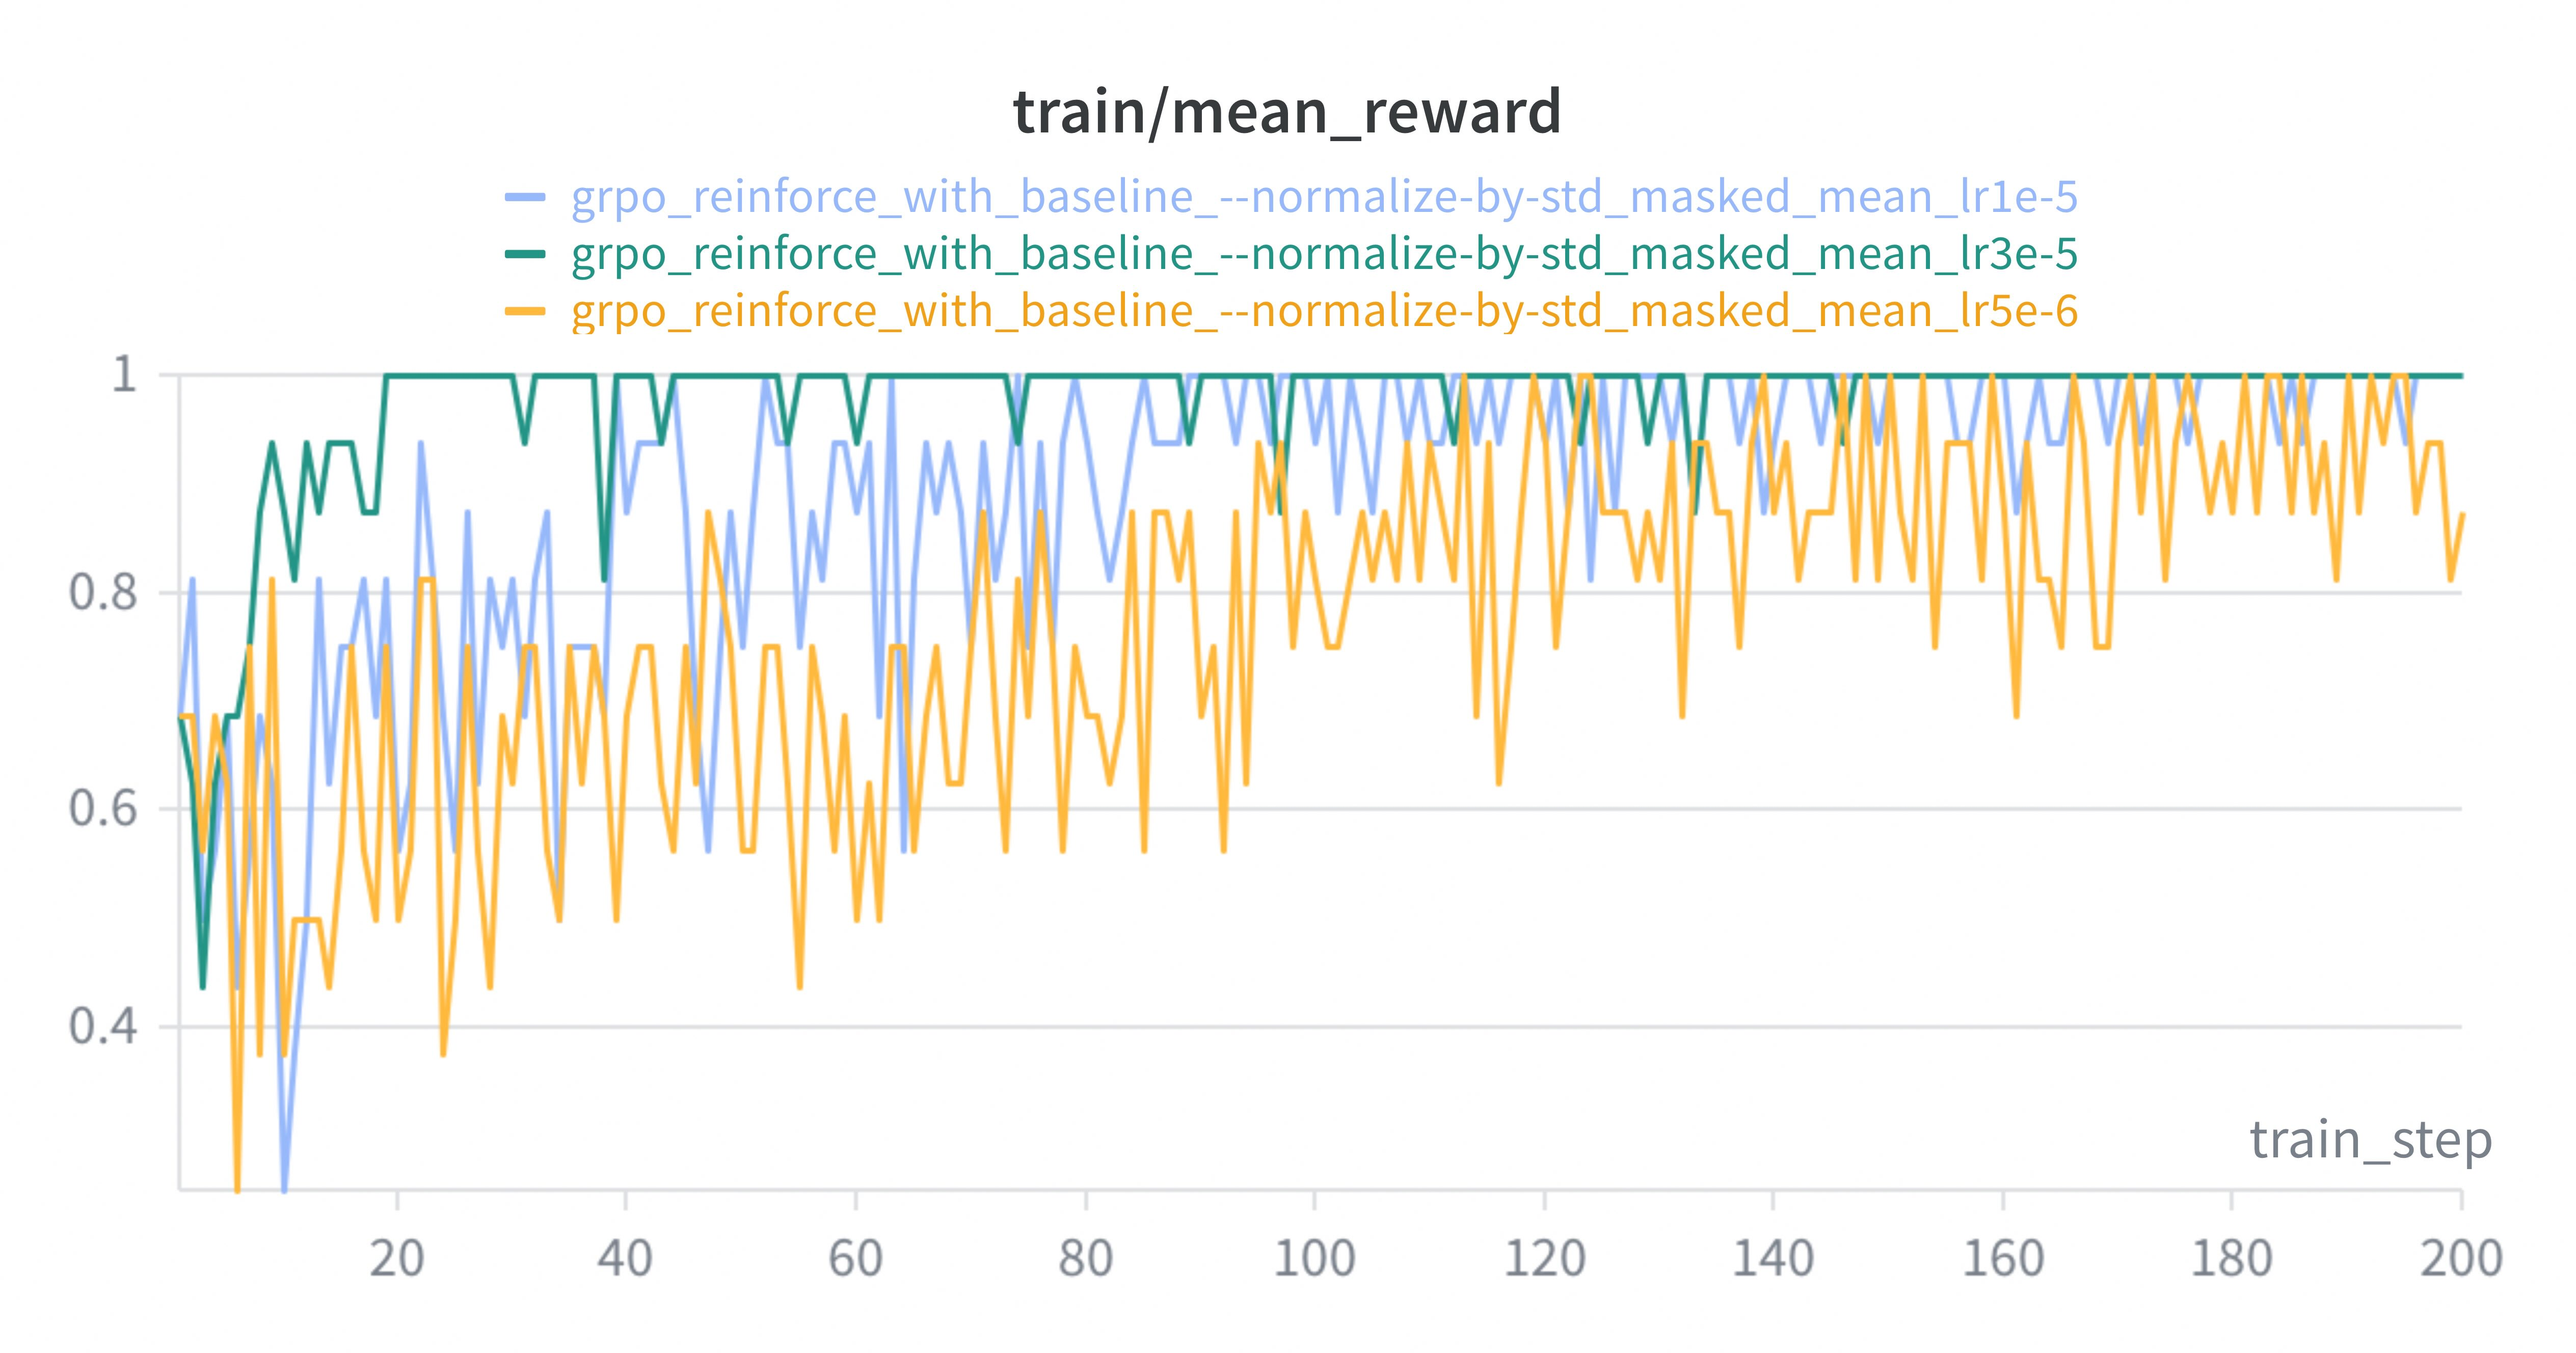
\includegraphics[width=0.9\linewidth]{../charts/grpo_lrs_experiment.jpg}
                \end{center}
            \item[\textbf{8.1.2}] \textbf{\texttt{grpo\_baseline}}\\
                The figures below show differences in \texttt{reinforce\_with\_baseline} and \texttt{no\_baseline} runs.
                \begin{center}
                    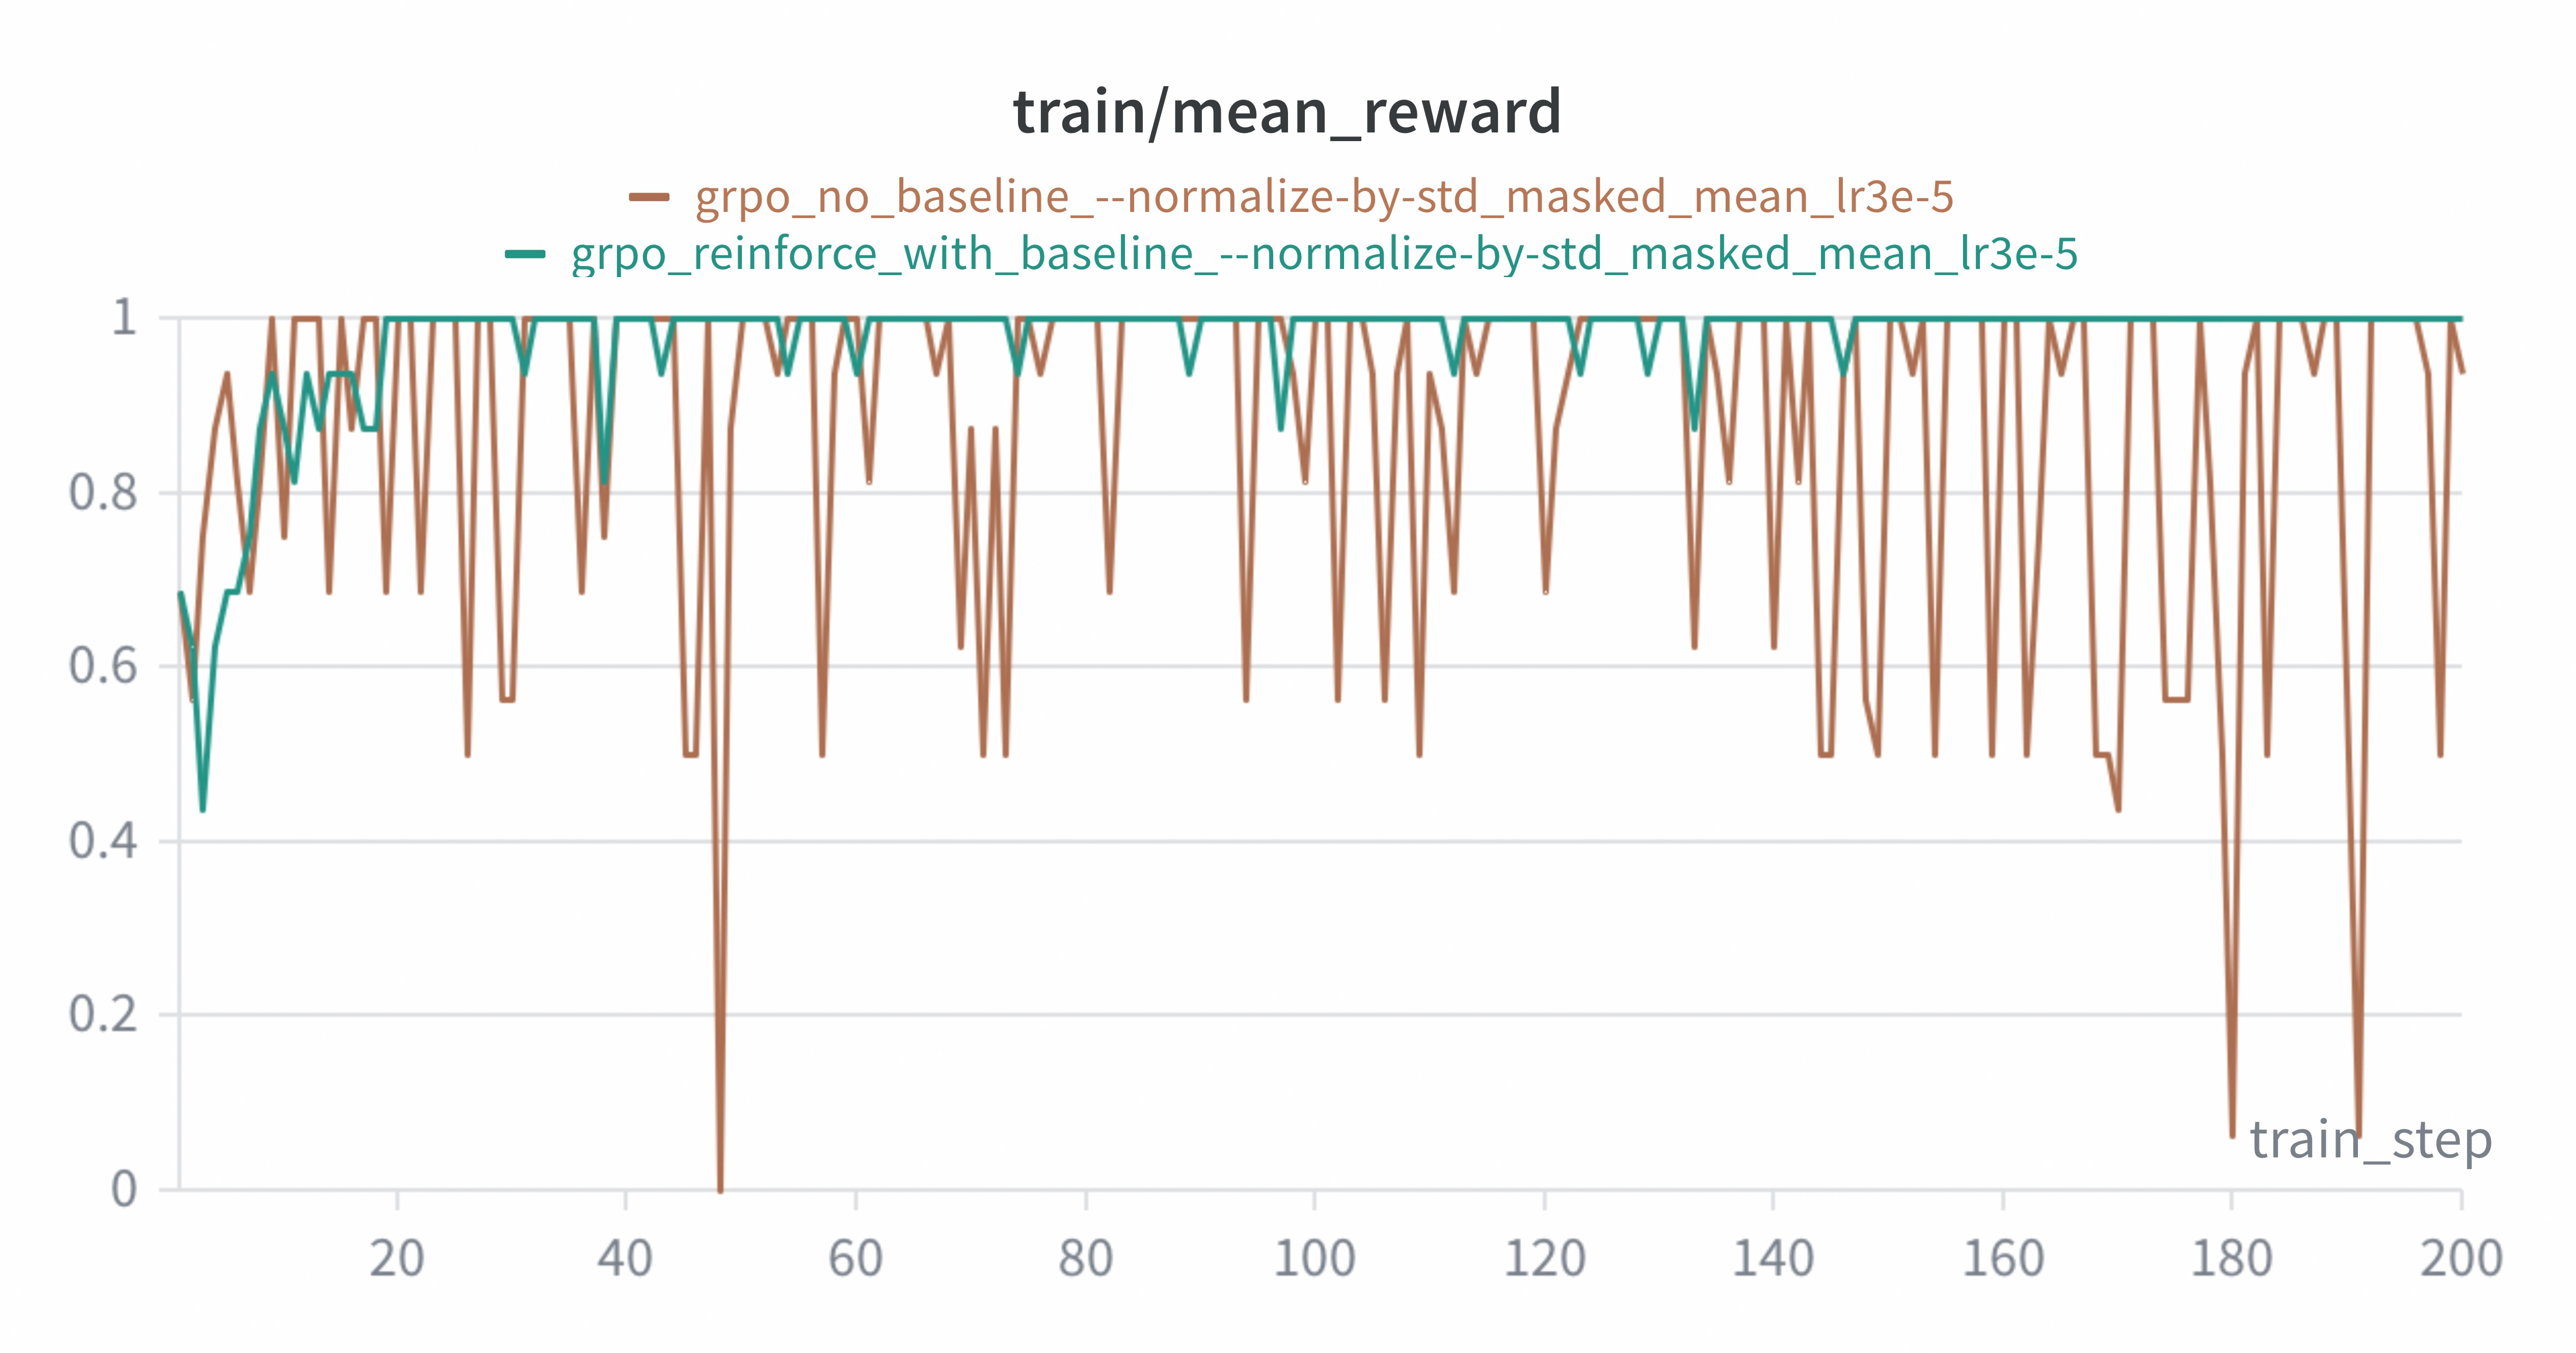
\includegraphics[width=0.9\linewidth]{../charts/grpo_no_baseline_reward_vs_step.jpg}
                    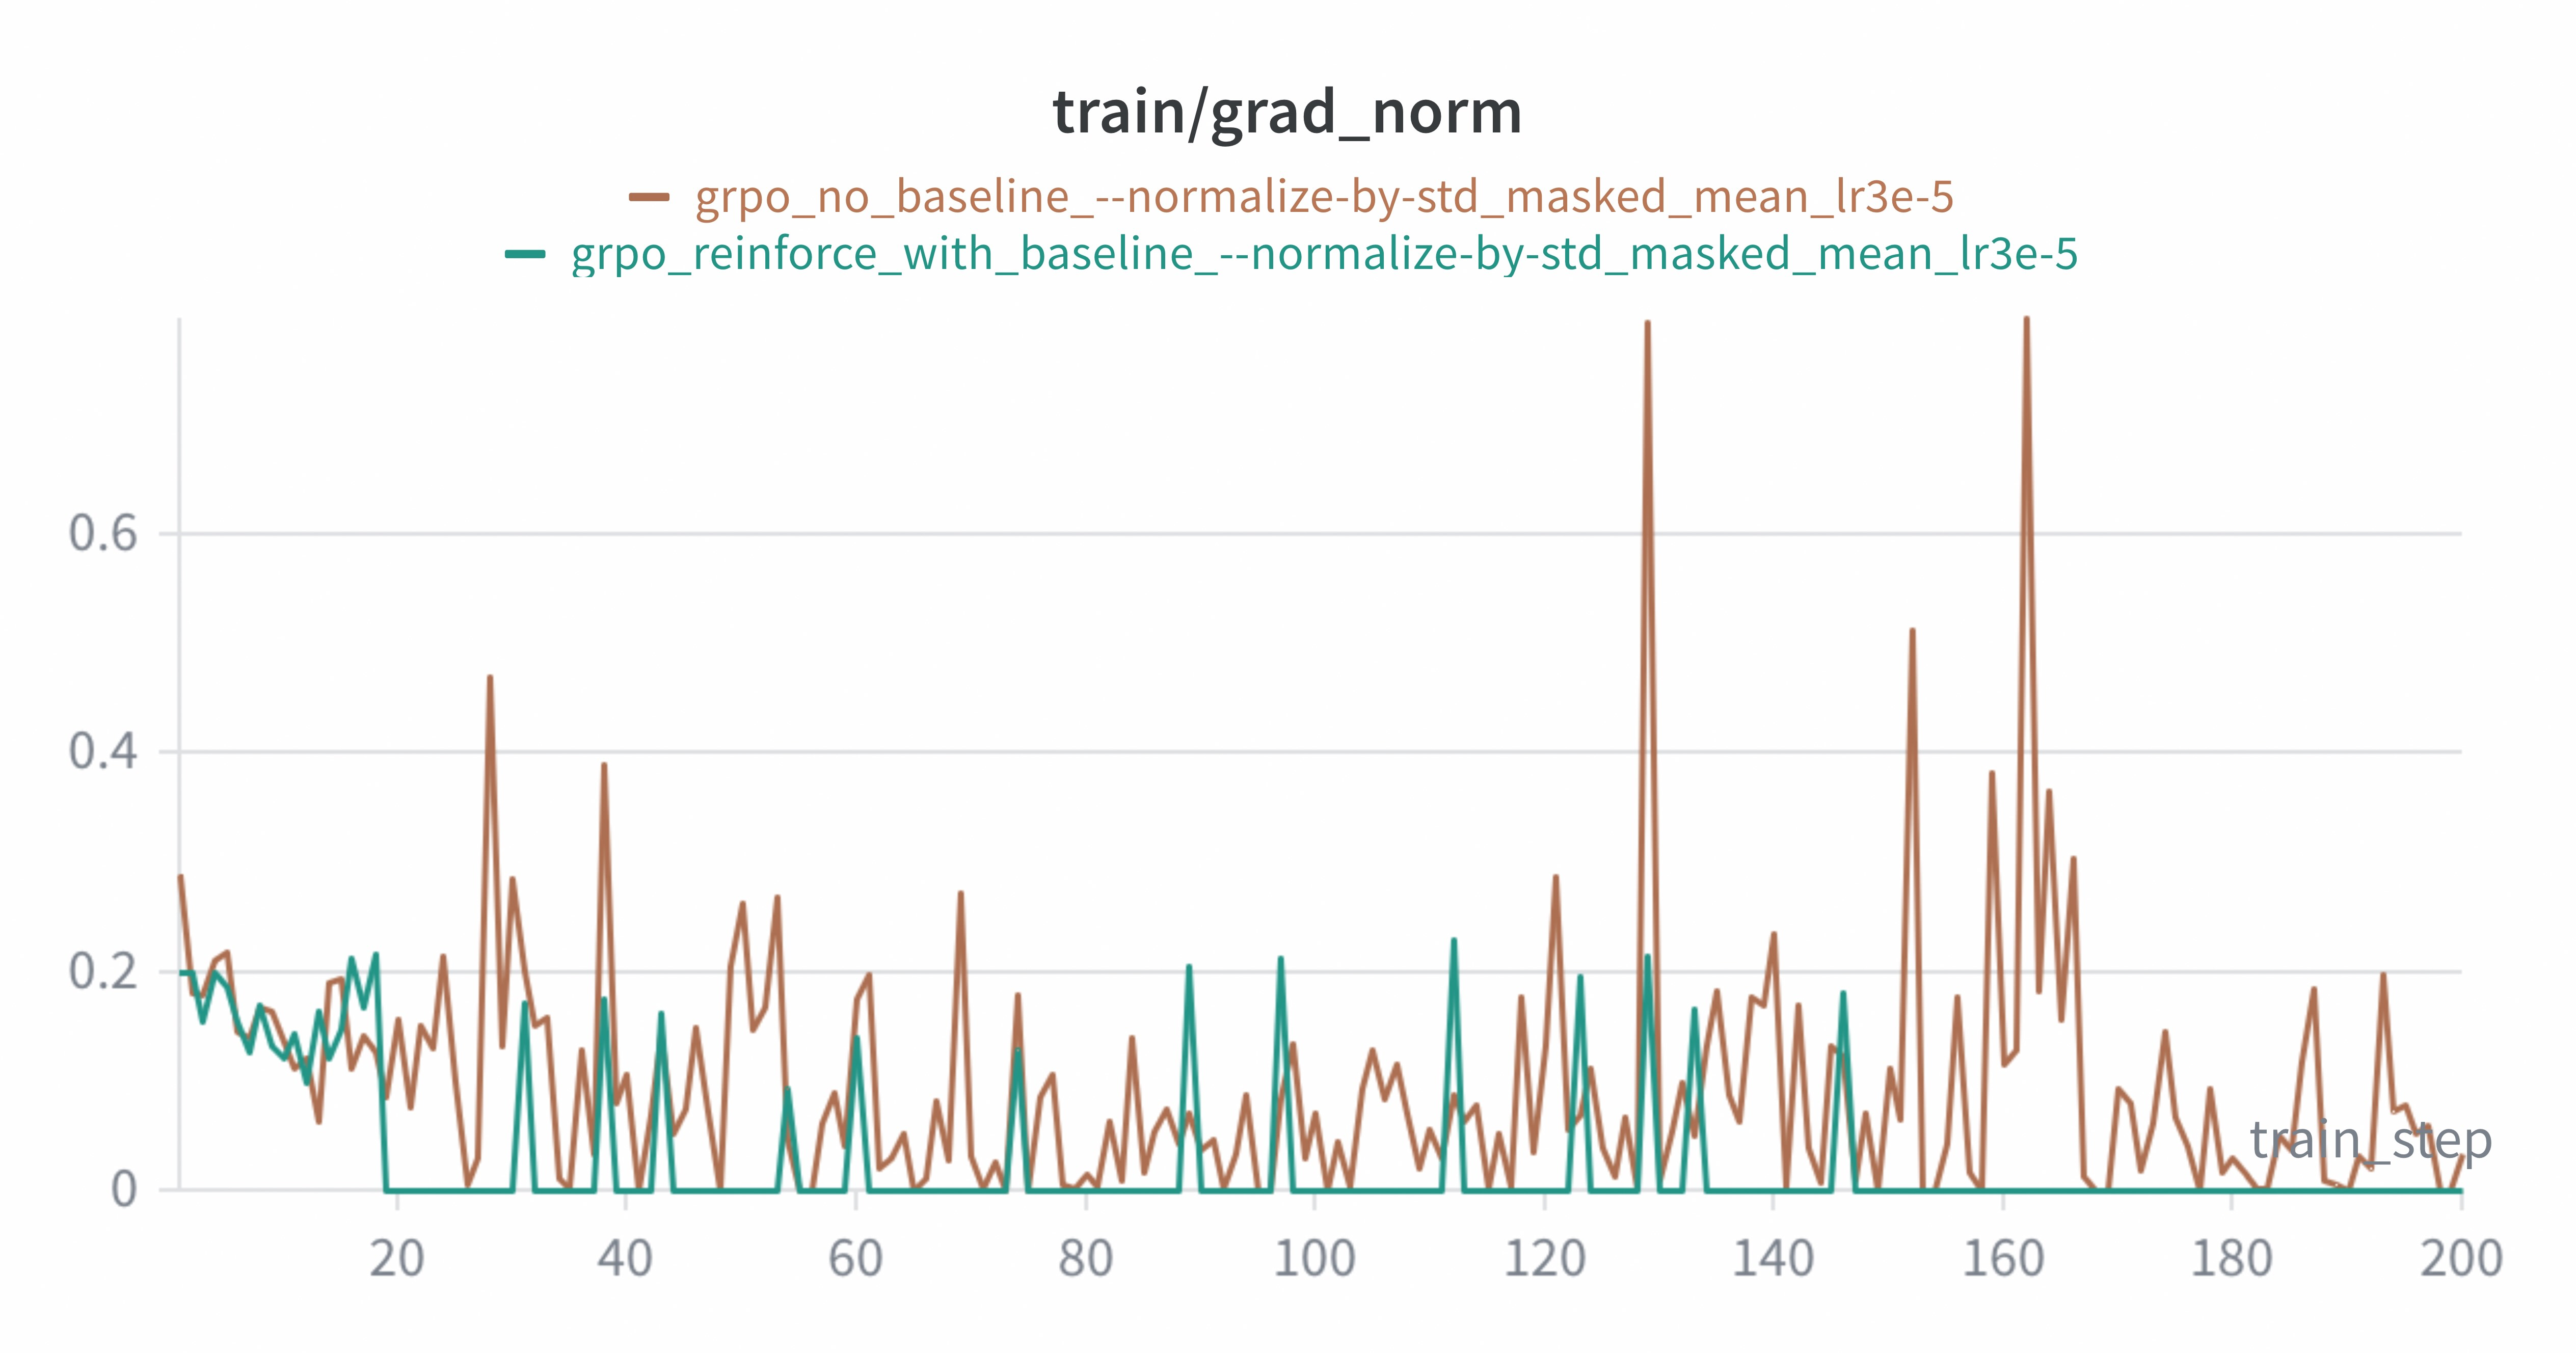
\includegraphics[width=0.9\linewidth]{../charts/grpo_no_baseline_grad_norm.jpg}
                    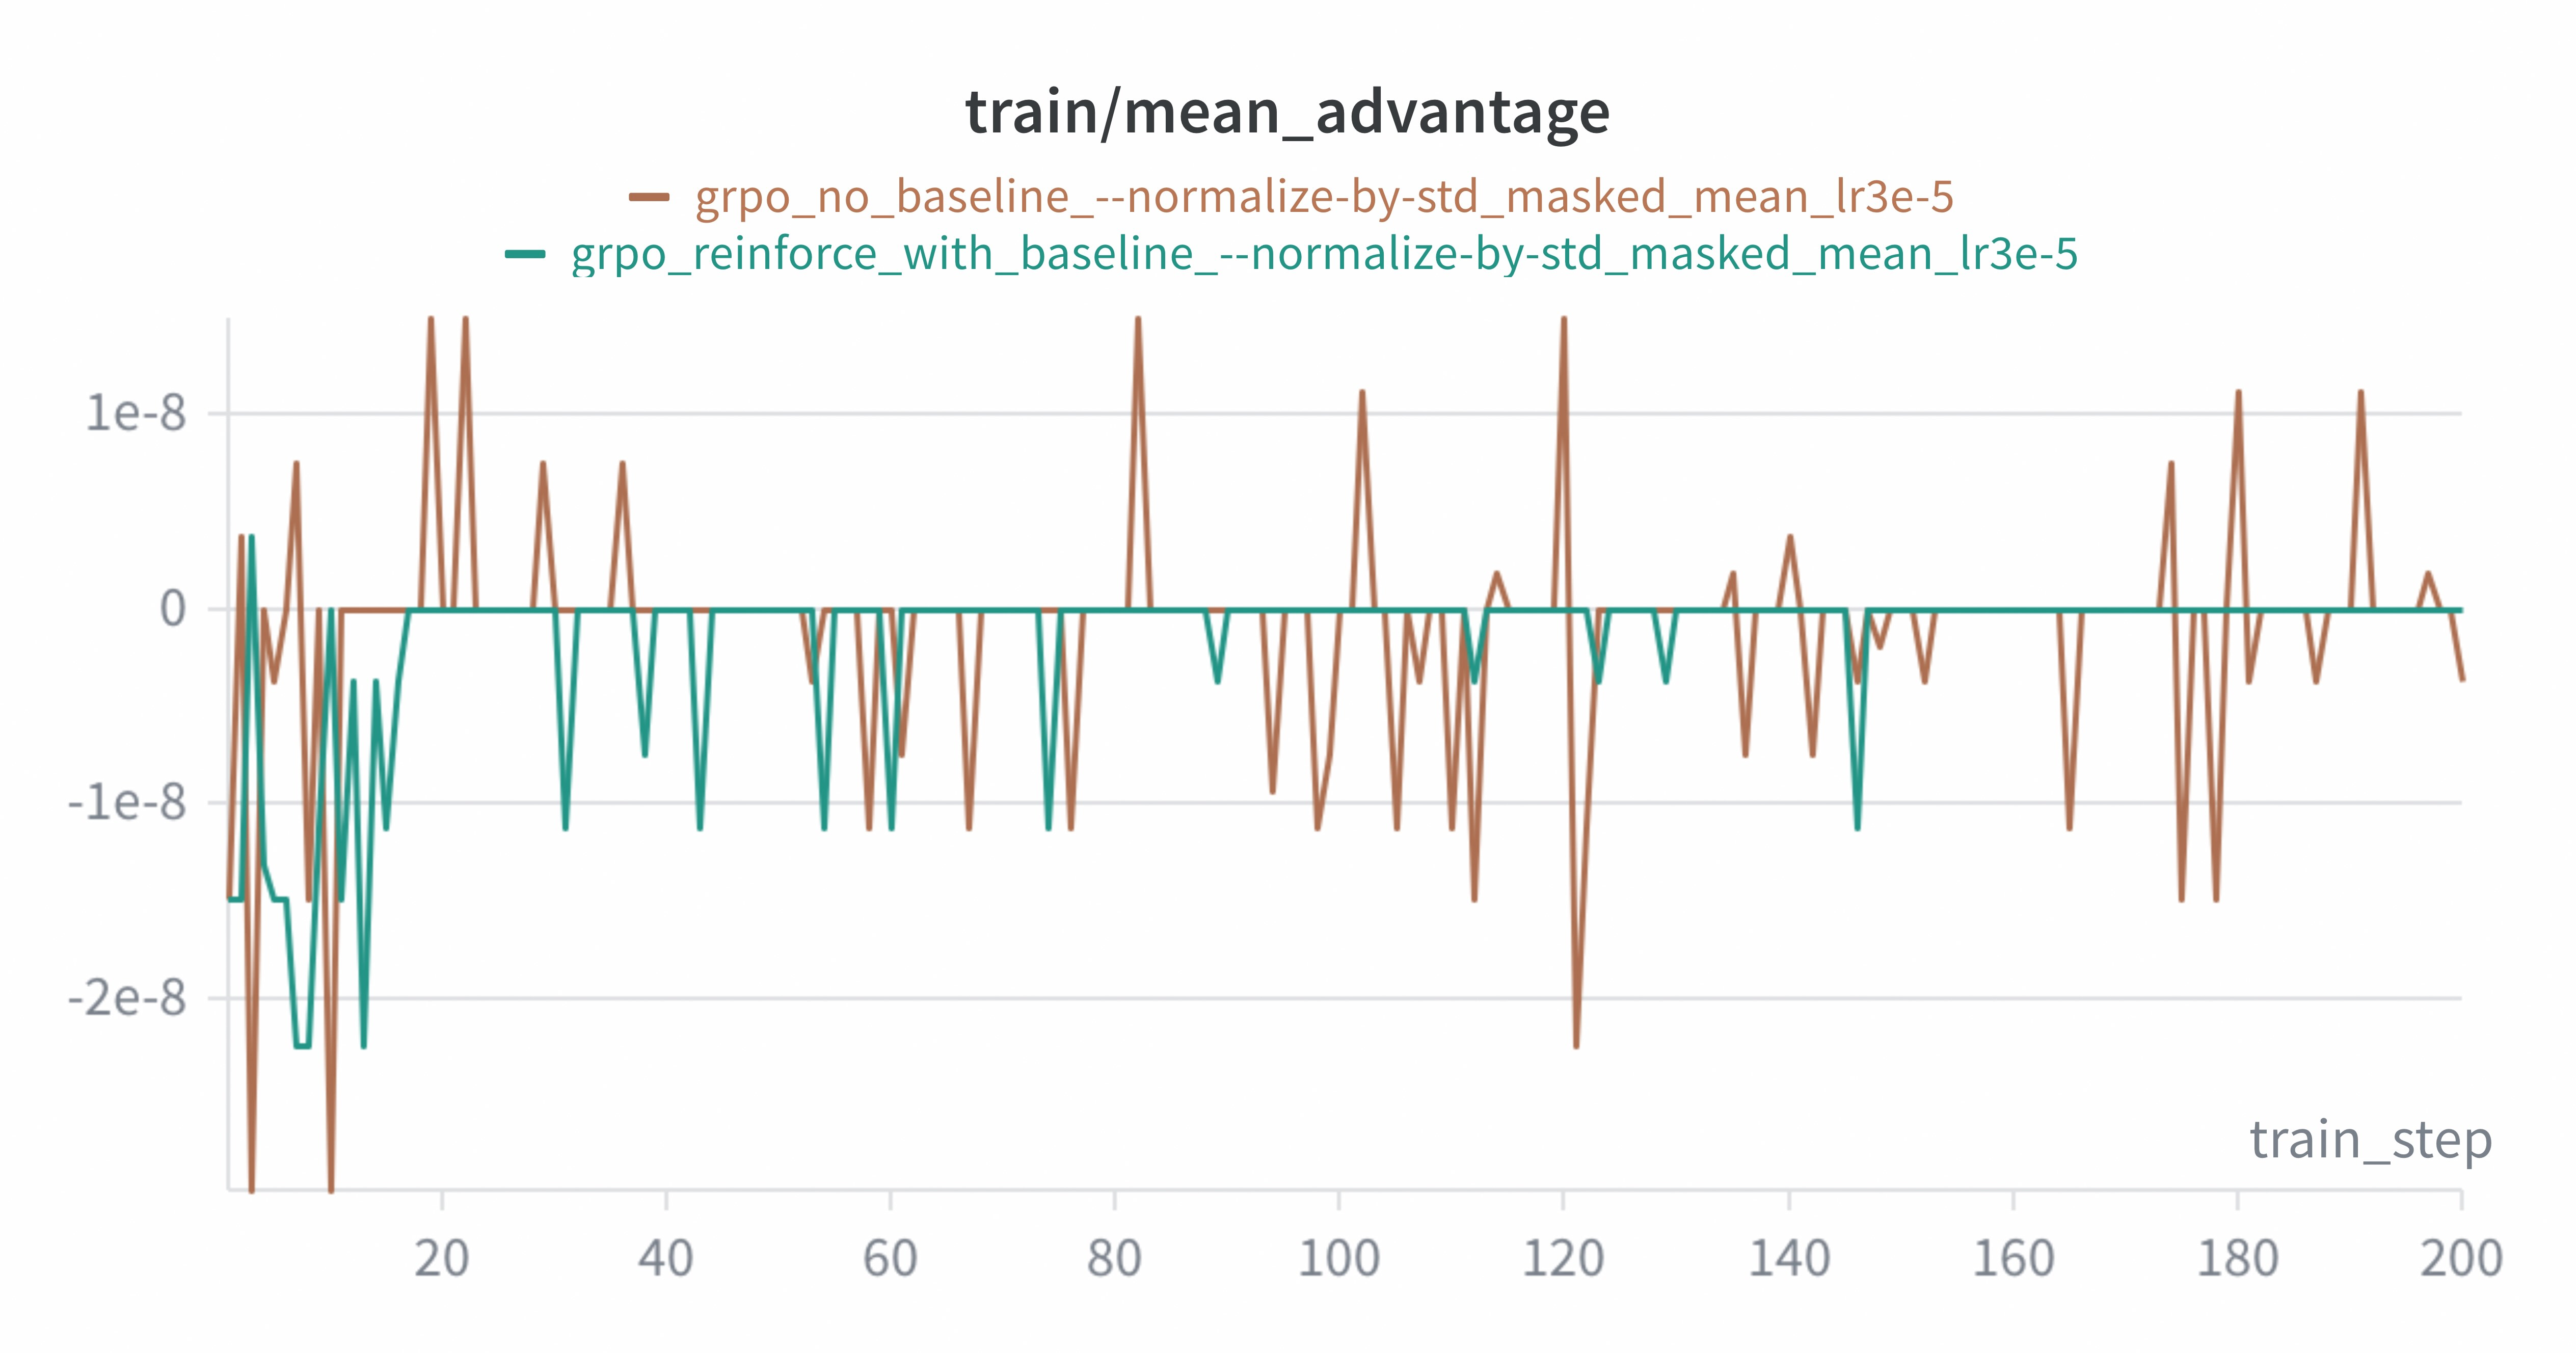
\includegraphics[width=0.9\linewidth]{../charts/grpo_no_baseline_adv.jpg}
                \end{center}
                We can see that the reward increase for the \texttt{no\_baseline} run is much more unstable compared to the \texttt{reinforce\_with\_baseline} run, which shows a steady increase in reward over time. The gradient norm for the \texttt{no\_baseline} run is also much higher and more variable compared to the \texttt{reinforce\_with\_baseline} run, which has a lower and more stable gradient norm. The advantage values for the \texttt{no\_baseline} run are also much more variable and can take on much larger values compared to the \texttt{reinforce\_with\_baseline} run, which has smaller and more stable advantage values. Overall, these observations suggest that using a baseline in the REINFORCE algorithm can help stabilize training and lead to better performance.
            \item[\textbf{8.1.3}] \textbf{\texttt{think\_about\_length\_normalization}}\\
                \texttt{masked\_mean} averages over each sequence’s active tokens, so every completion contributes roughly equally regardless of length; this is usually more stable and reduces bias toward long responses, but it can under-credit long trajectories by shrinking their per-token signal.\\
                \texttt{masked\_normalize} sums over active tokens and divides by a fixed constant, which keeps per-token scaling more uniform across samples and can preserve stronger token-level credit assignment, but it tends to make total update magnitude more length-dependent and can increase optimization volatility.\\
                In settings with high length variation or where long chains of reasoning should receive proportionally more total credit, \texttt{masked\_normalize} can be preferable, while in tasks like Countdown (shorter outputs, equal-example weighting) \texttt{masked\_mean} is often the safer default.
            \item[\textbf{8.1.4}] \textbf{\texttt{grpo\_length\_normalization}}\\
                The figures below show differences in \texttt{masked\_mean} and \texttt{masked\_normalize} normalization runs.
                \begin{center}
                    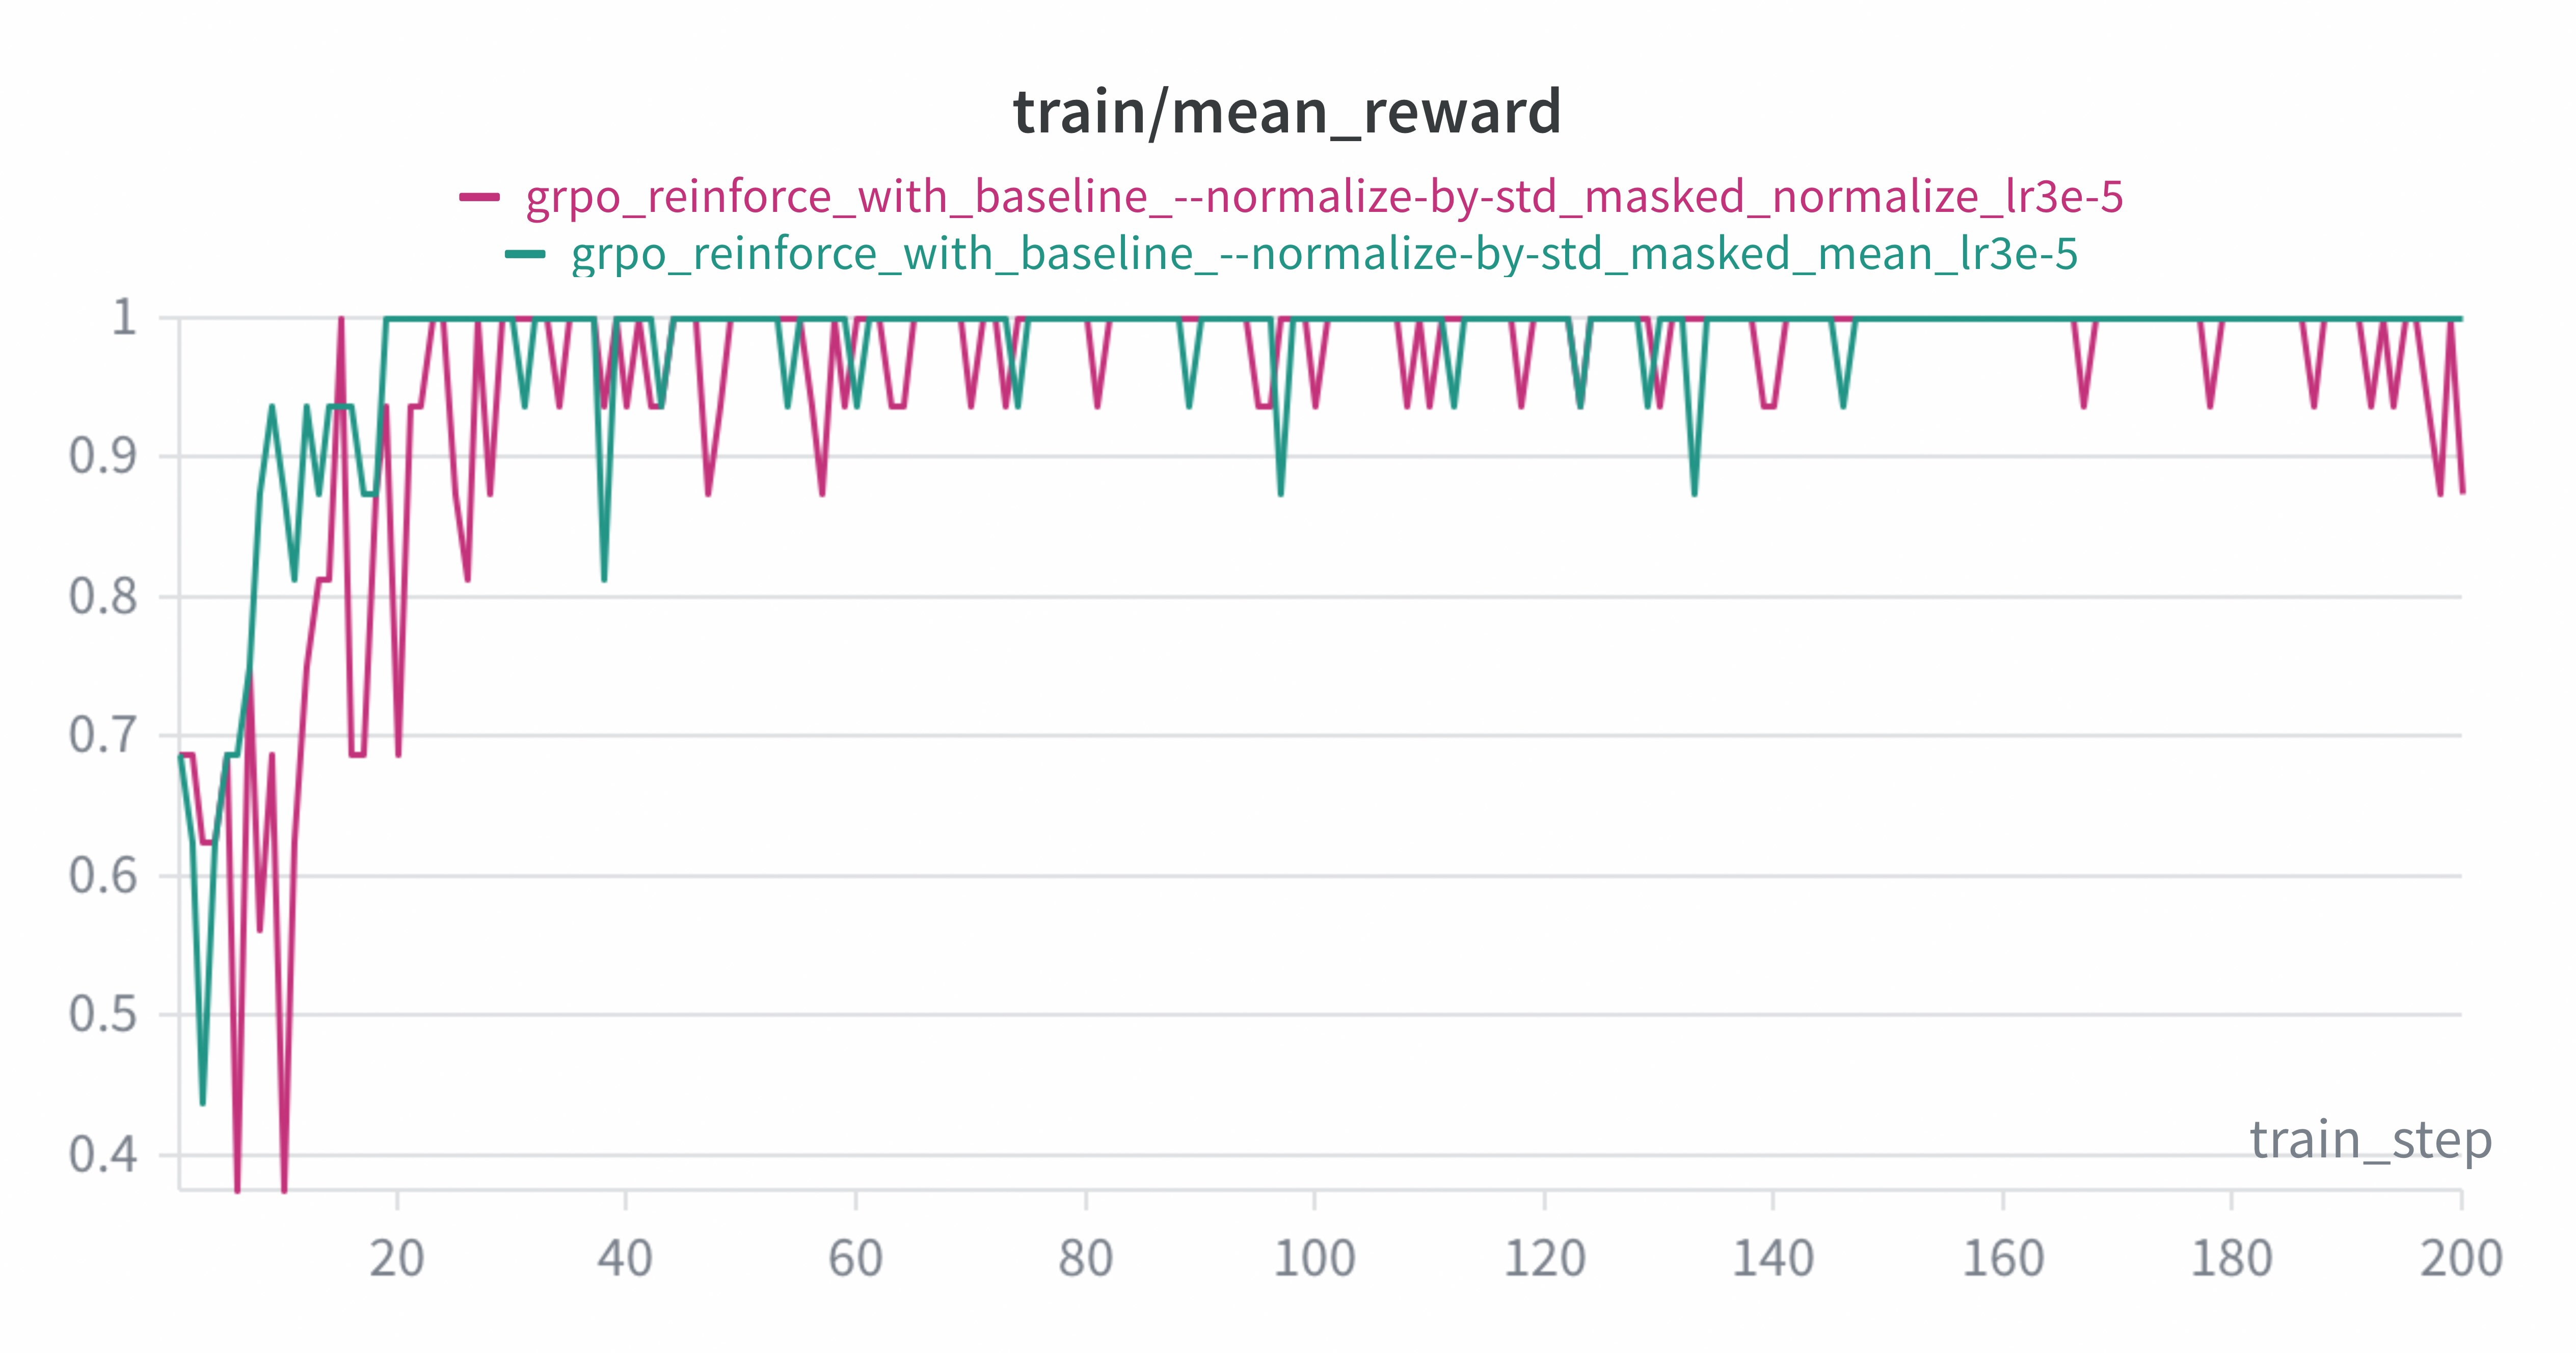
\includegraphics[width=0.9\linewidth]{../charts/grpo_length_norm_reward_vs_step.jpg}
                    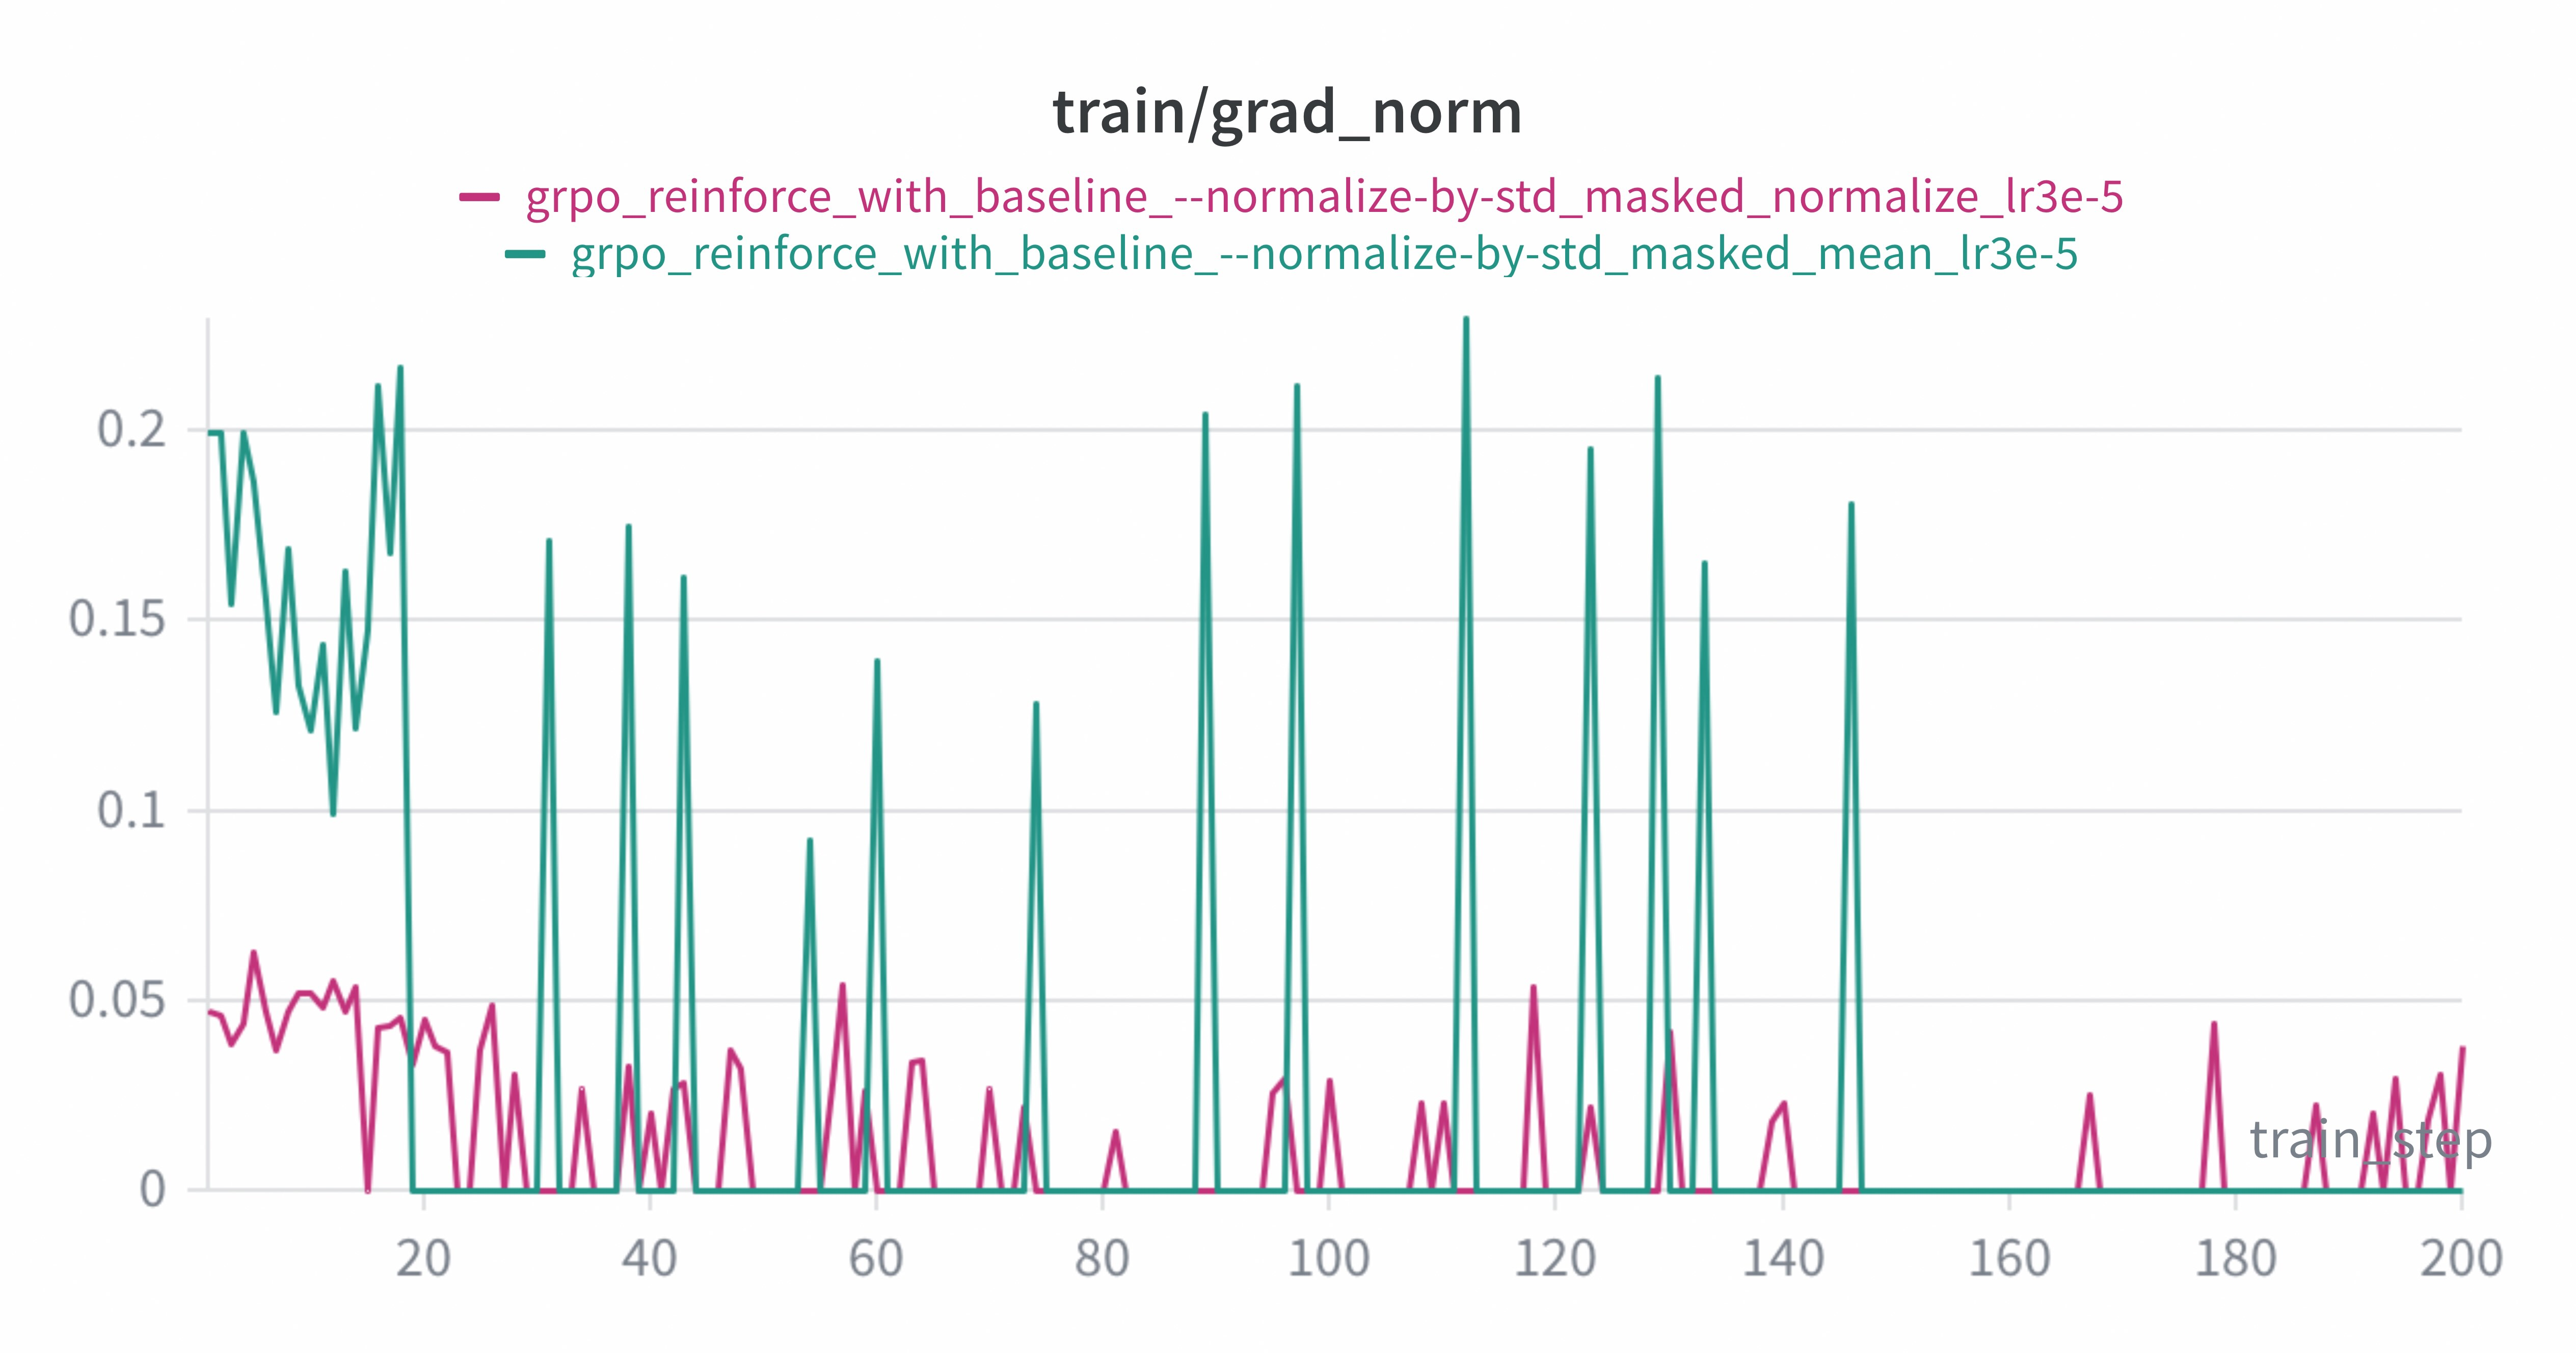
\includegraphics[width=0.9\linewidth]{../charts/grpo_length_norm_grad_norm.jpg}
                    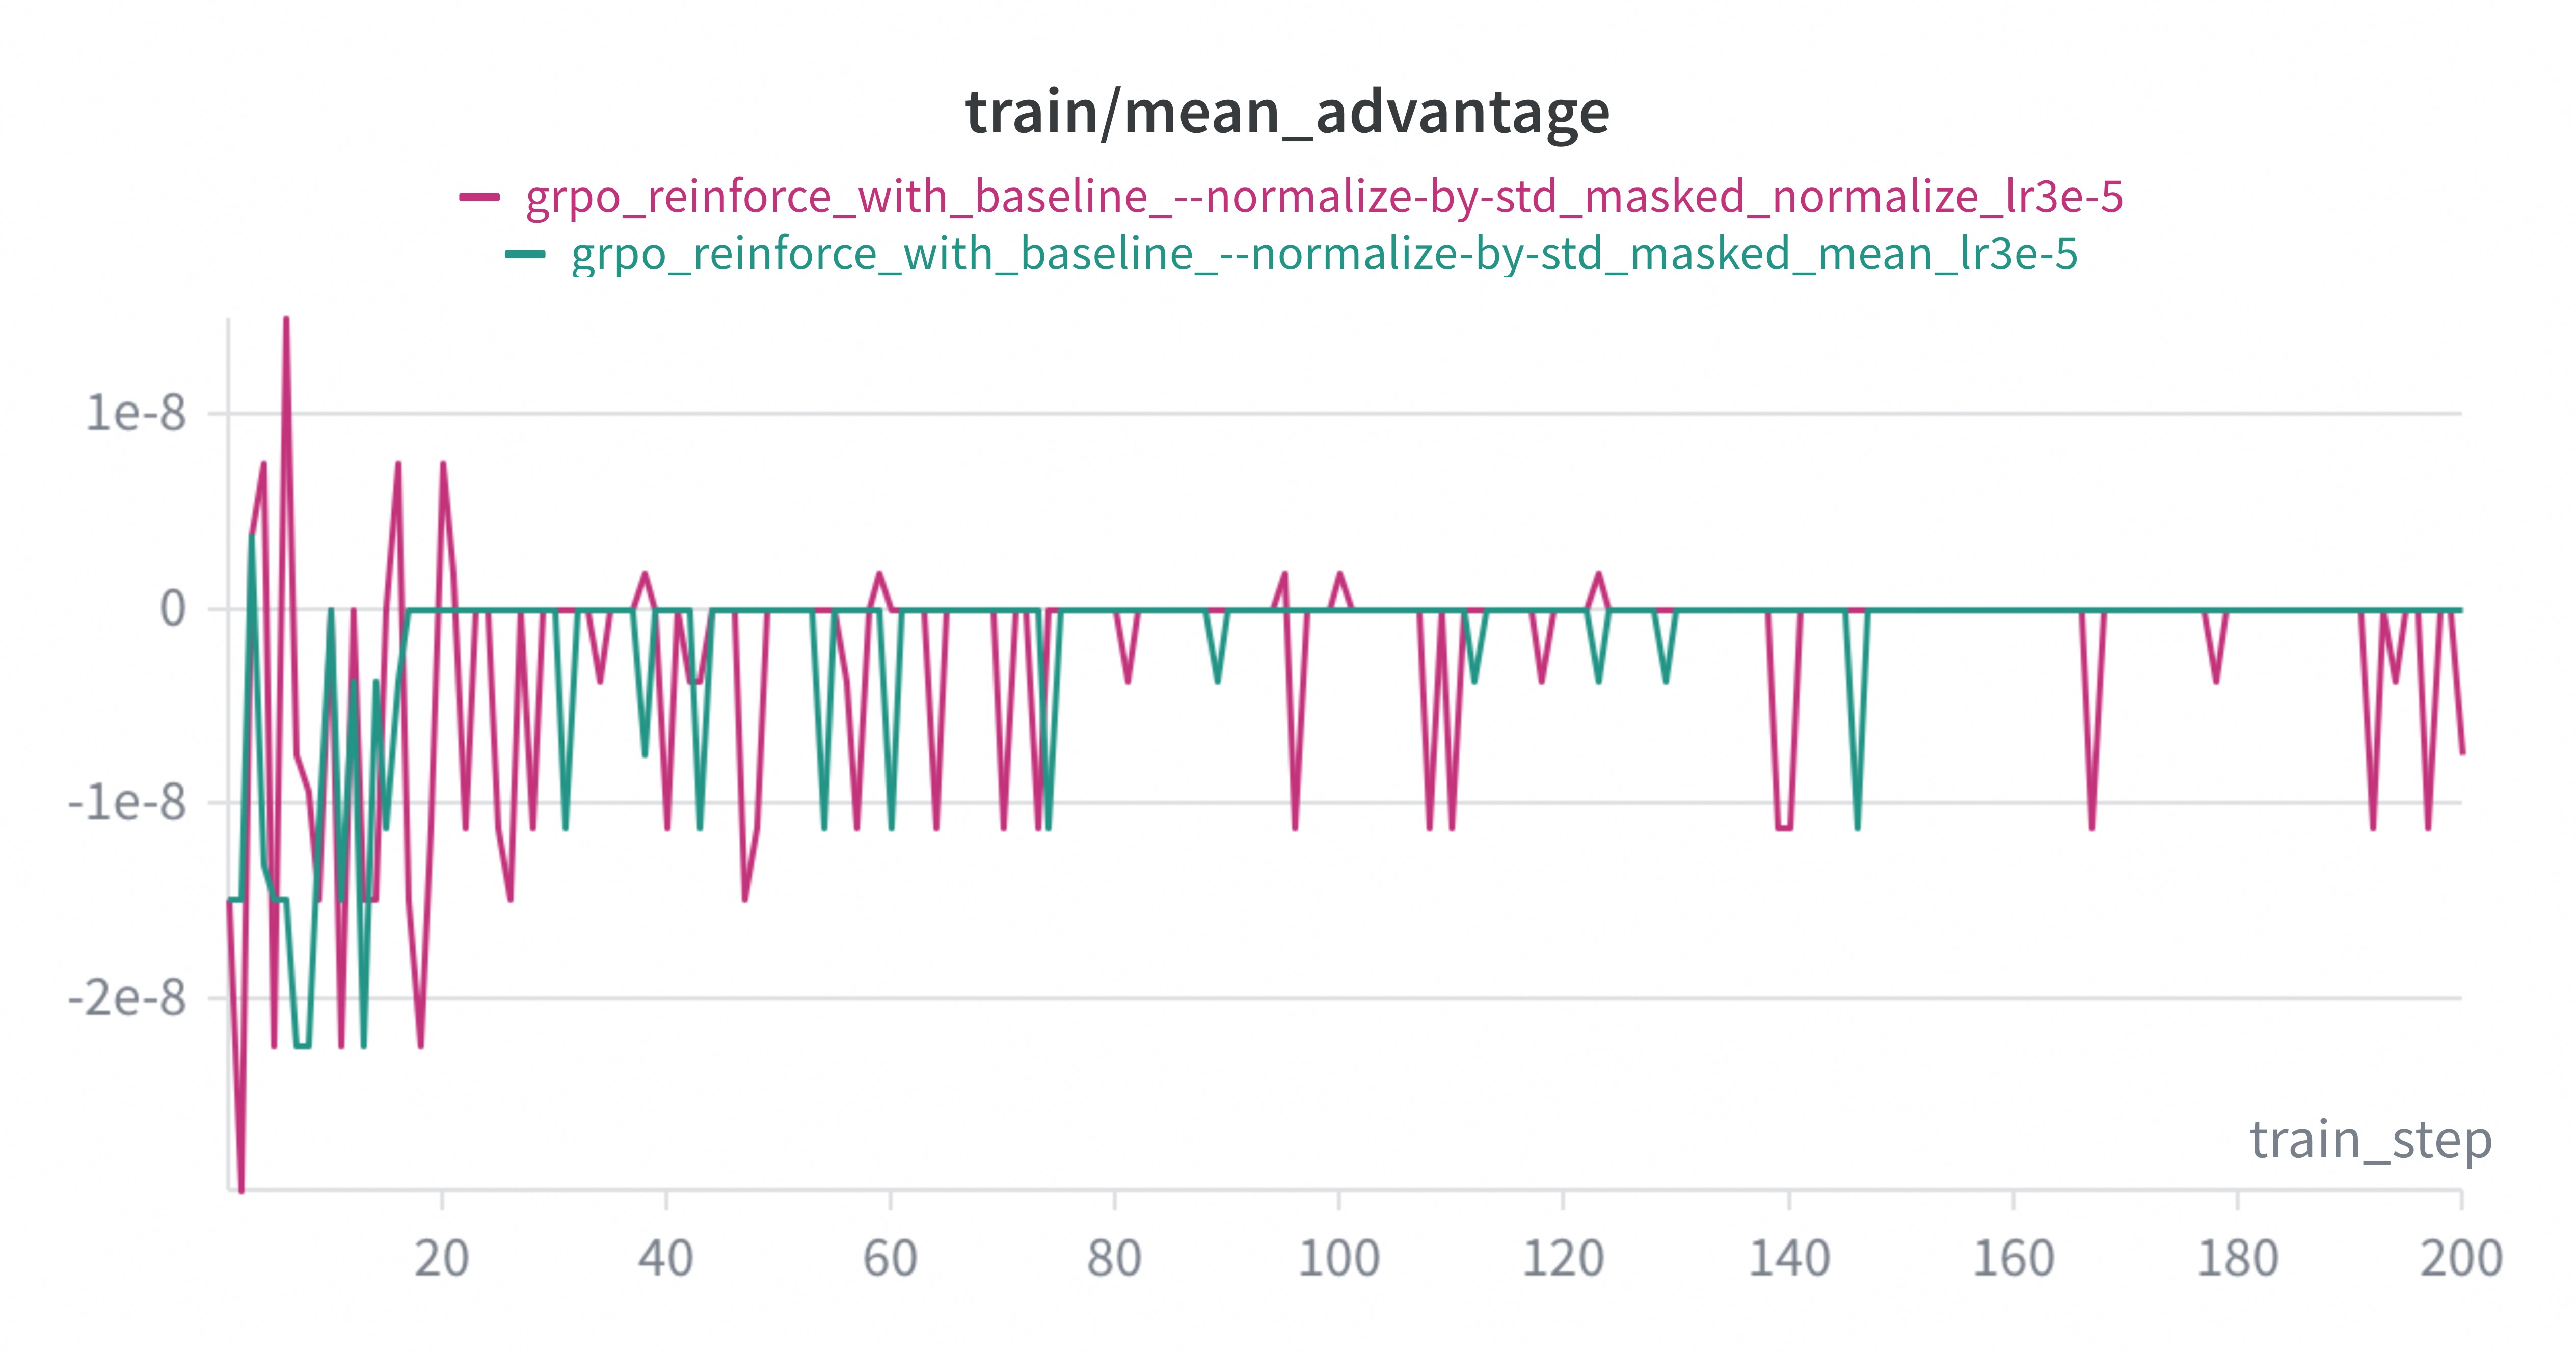
\includegraphics[width=0.9\linewidth]{../charts/grpo_length_norm_adv.jpg}
                \end{center}
                We can see that the reward increase for the \texttt{masked\_mean} and \texttt{masked\_normalize} runs are mostly similar but the \texttt{masked\_mean} run shows a slightly faster increase and stability. The gradient norm for the \texttt{masked\_normalize} run seems low compared to the \texttt{masked\_mean} run, but the number of variations across training is higher for the \texttt{masked\_normalize} run. The \texttt{masked\_mean} run had a higher overall gradient norm level, while \texttt{masked\_normalize} showed more frequent short spikes and a few late-training reward spikes, which suggests it is somewhat more sensitive to batch-to-batch variation. The advantage values for the \texttt{masked\_normalize} normalization run are more variable and can take on larger values compared to the \texttt{masked\_mean} run, especially towards the end of training.
            \item[\textbf{8.1.5}] \textbf{\texttt{grpo\_group\_standard\_deviation}}\\
                The figures below show differences in \texttt{use\_std\_normalization == True} and \texttt{use\_std\_normalization == False} runs.
                \begin{center}
                    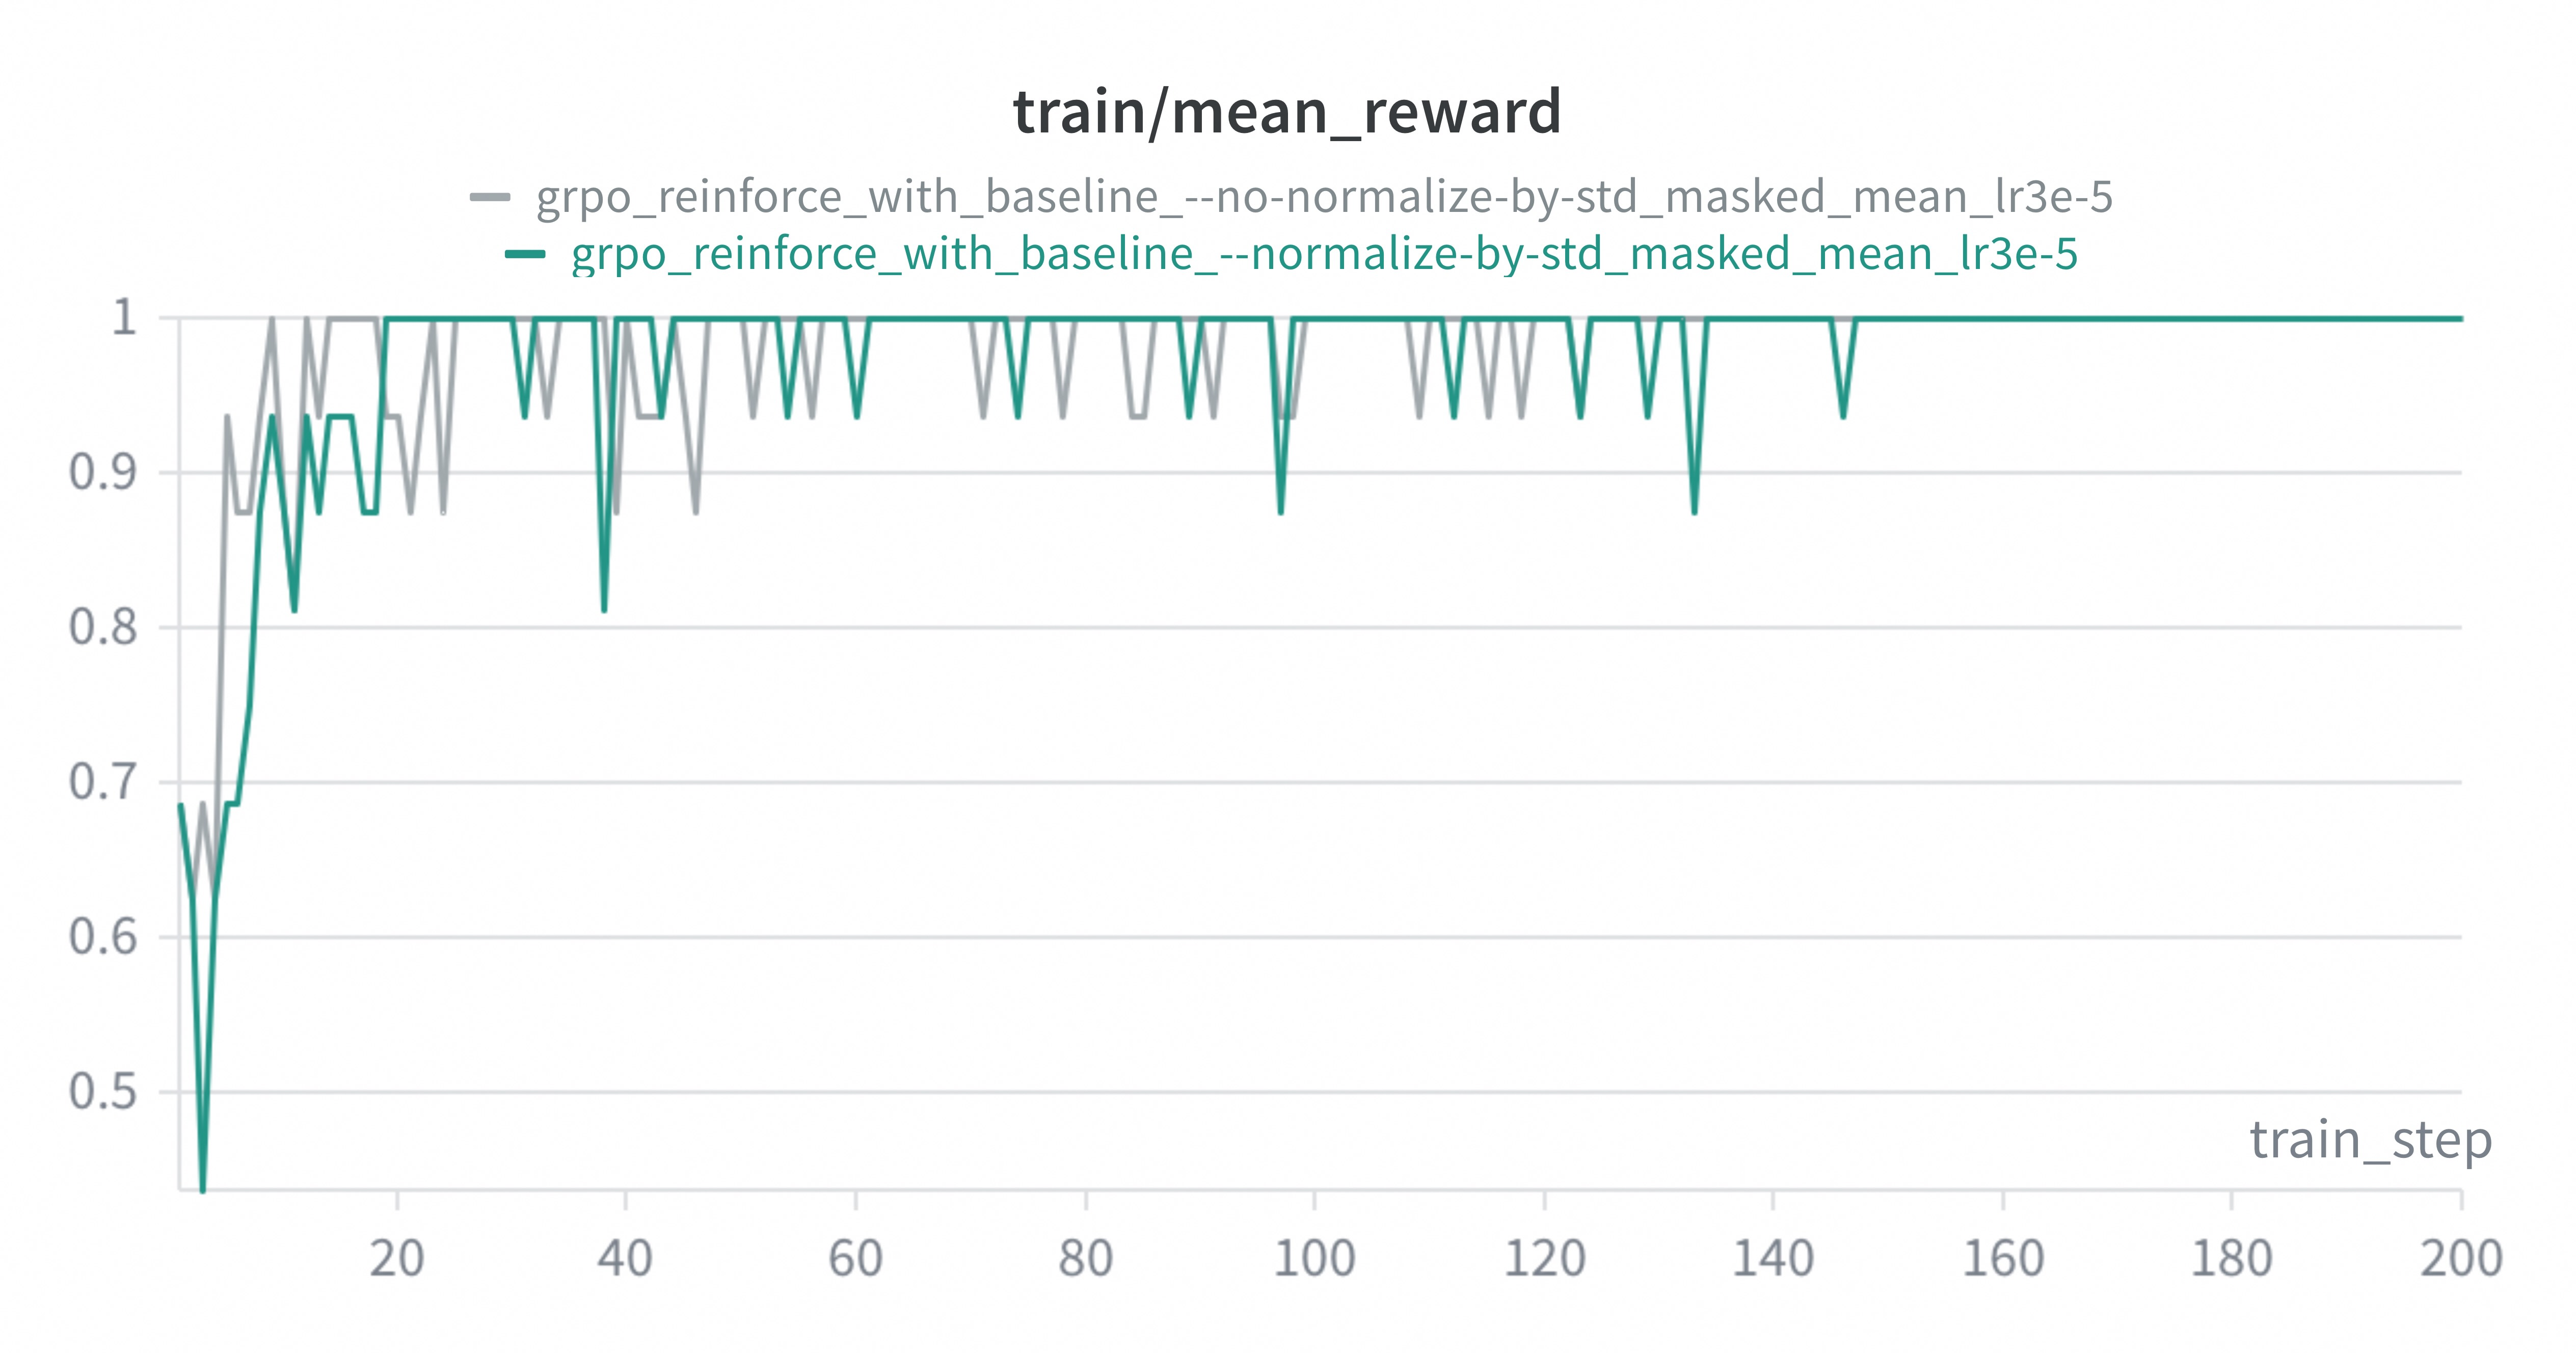
\includegraphics[width=0.9\linewidth]{../charts/grpo_no_std_reward_vs_step.jpg}
                    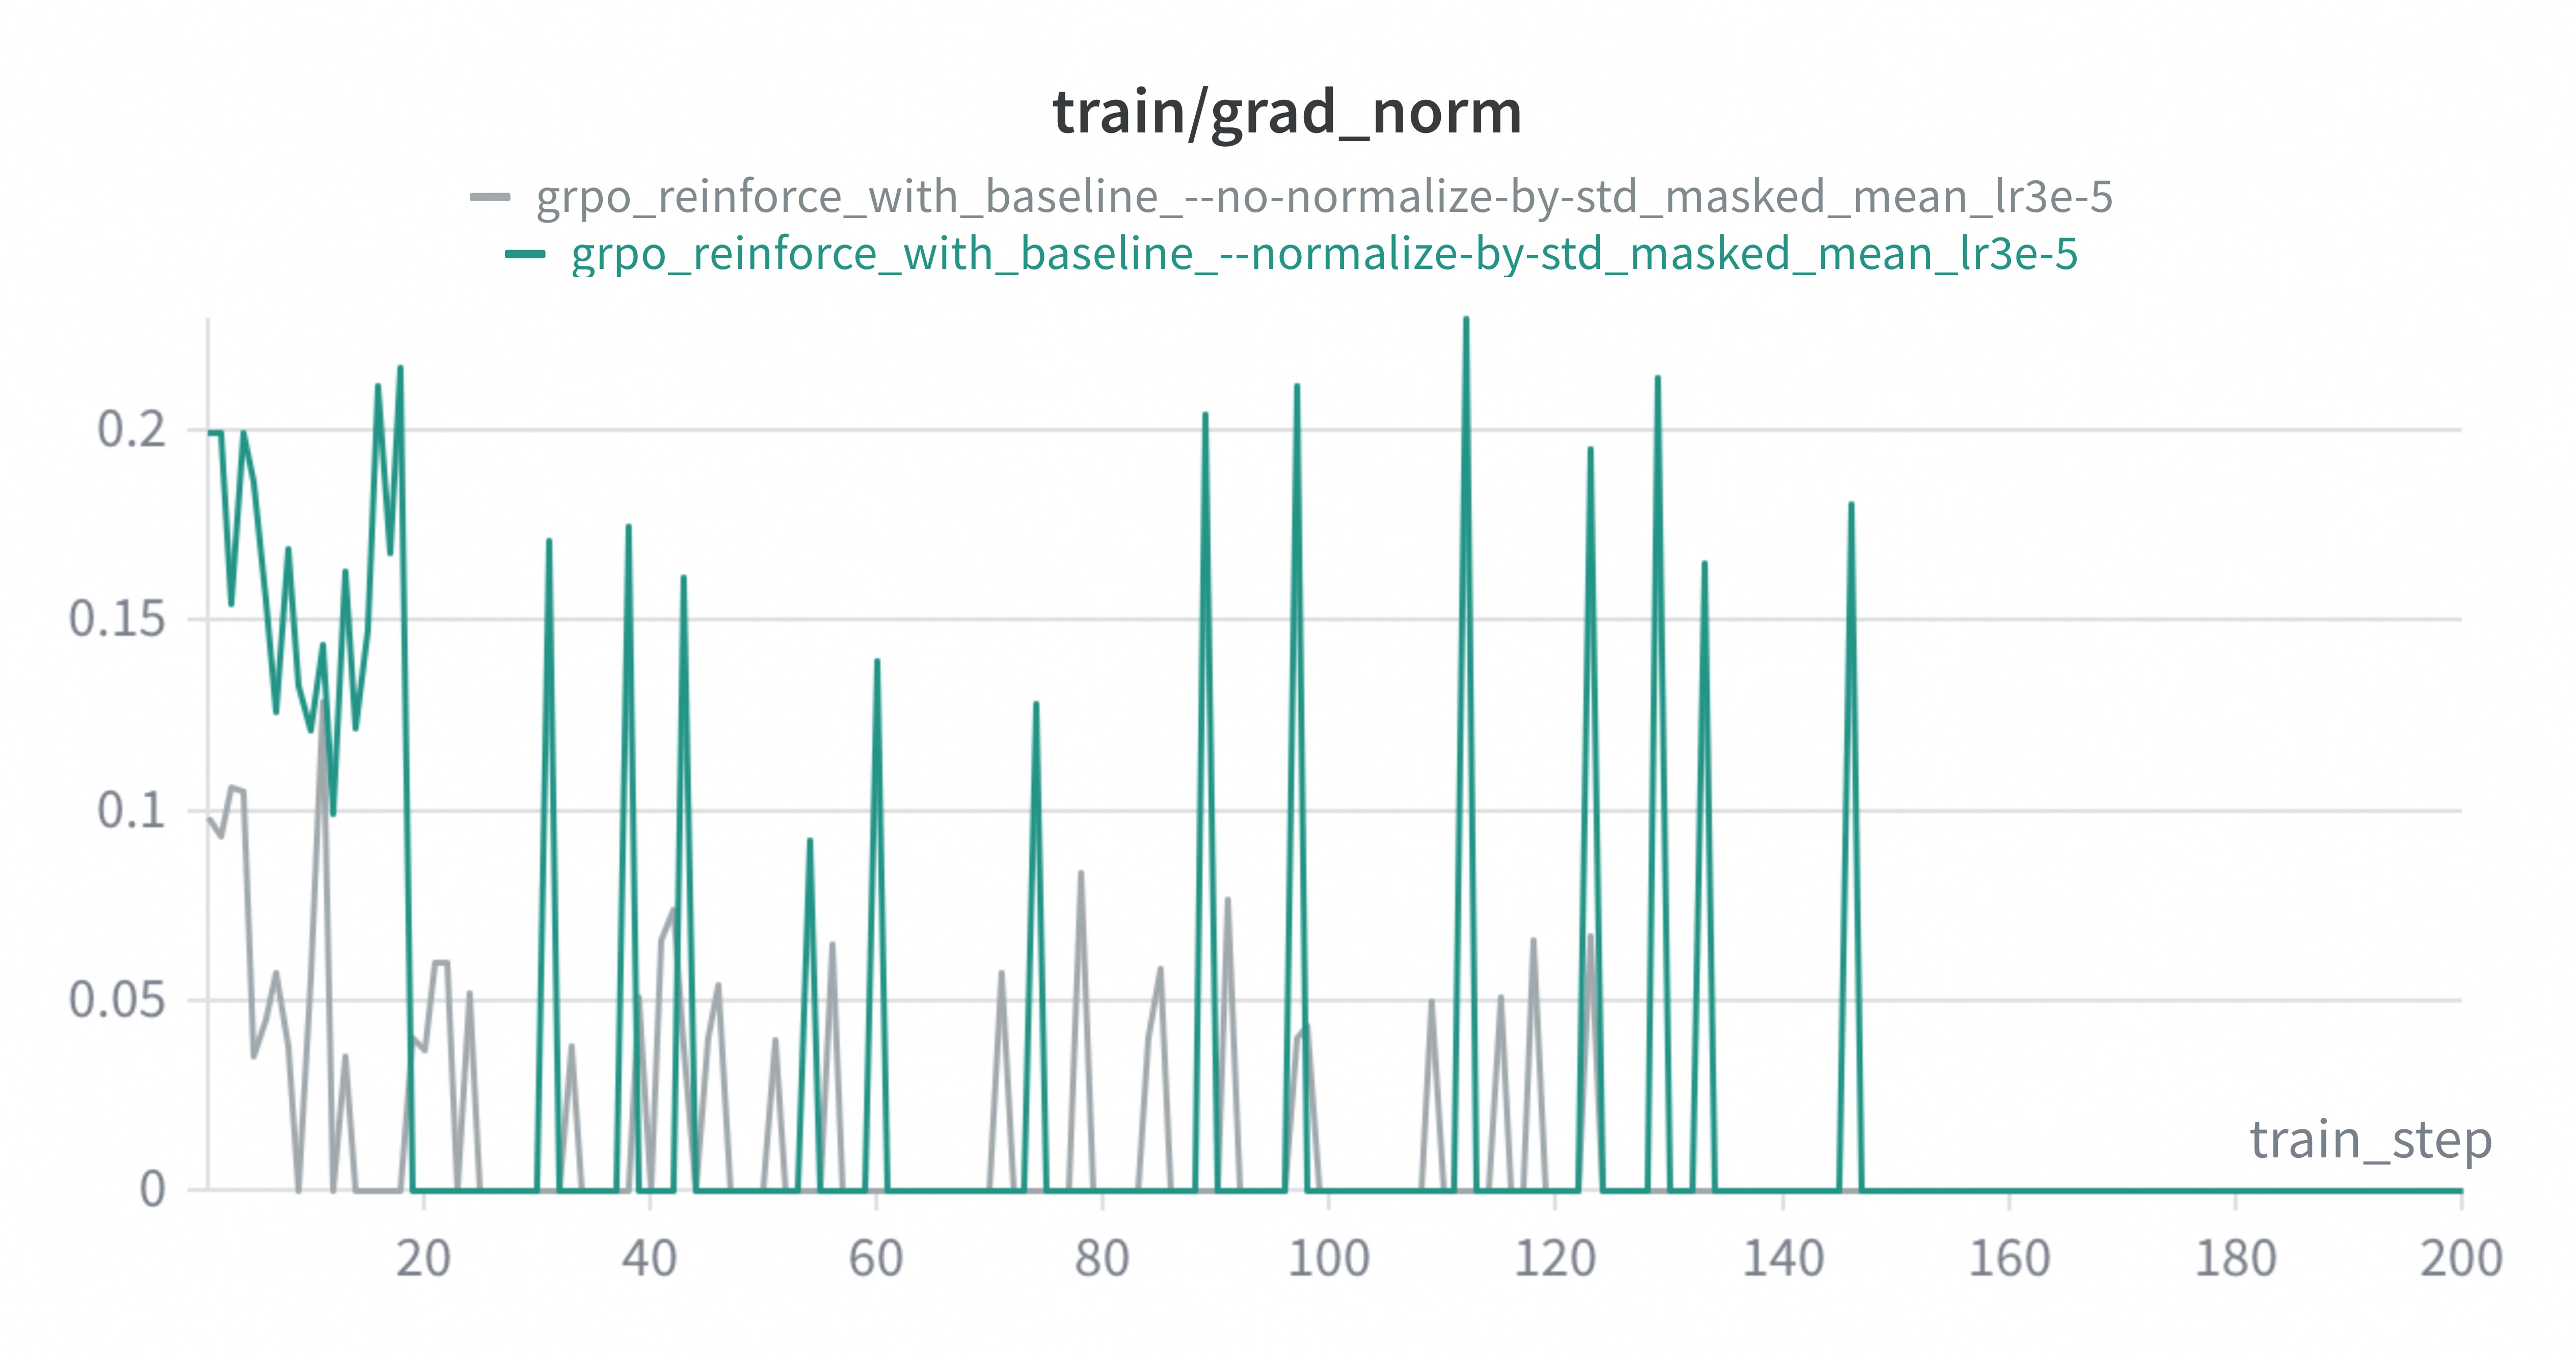
\includegraphics[width=0.9\linewidth]{../charts/grpo_no_std_grad_norm.jpg}
                    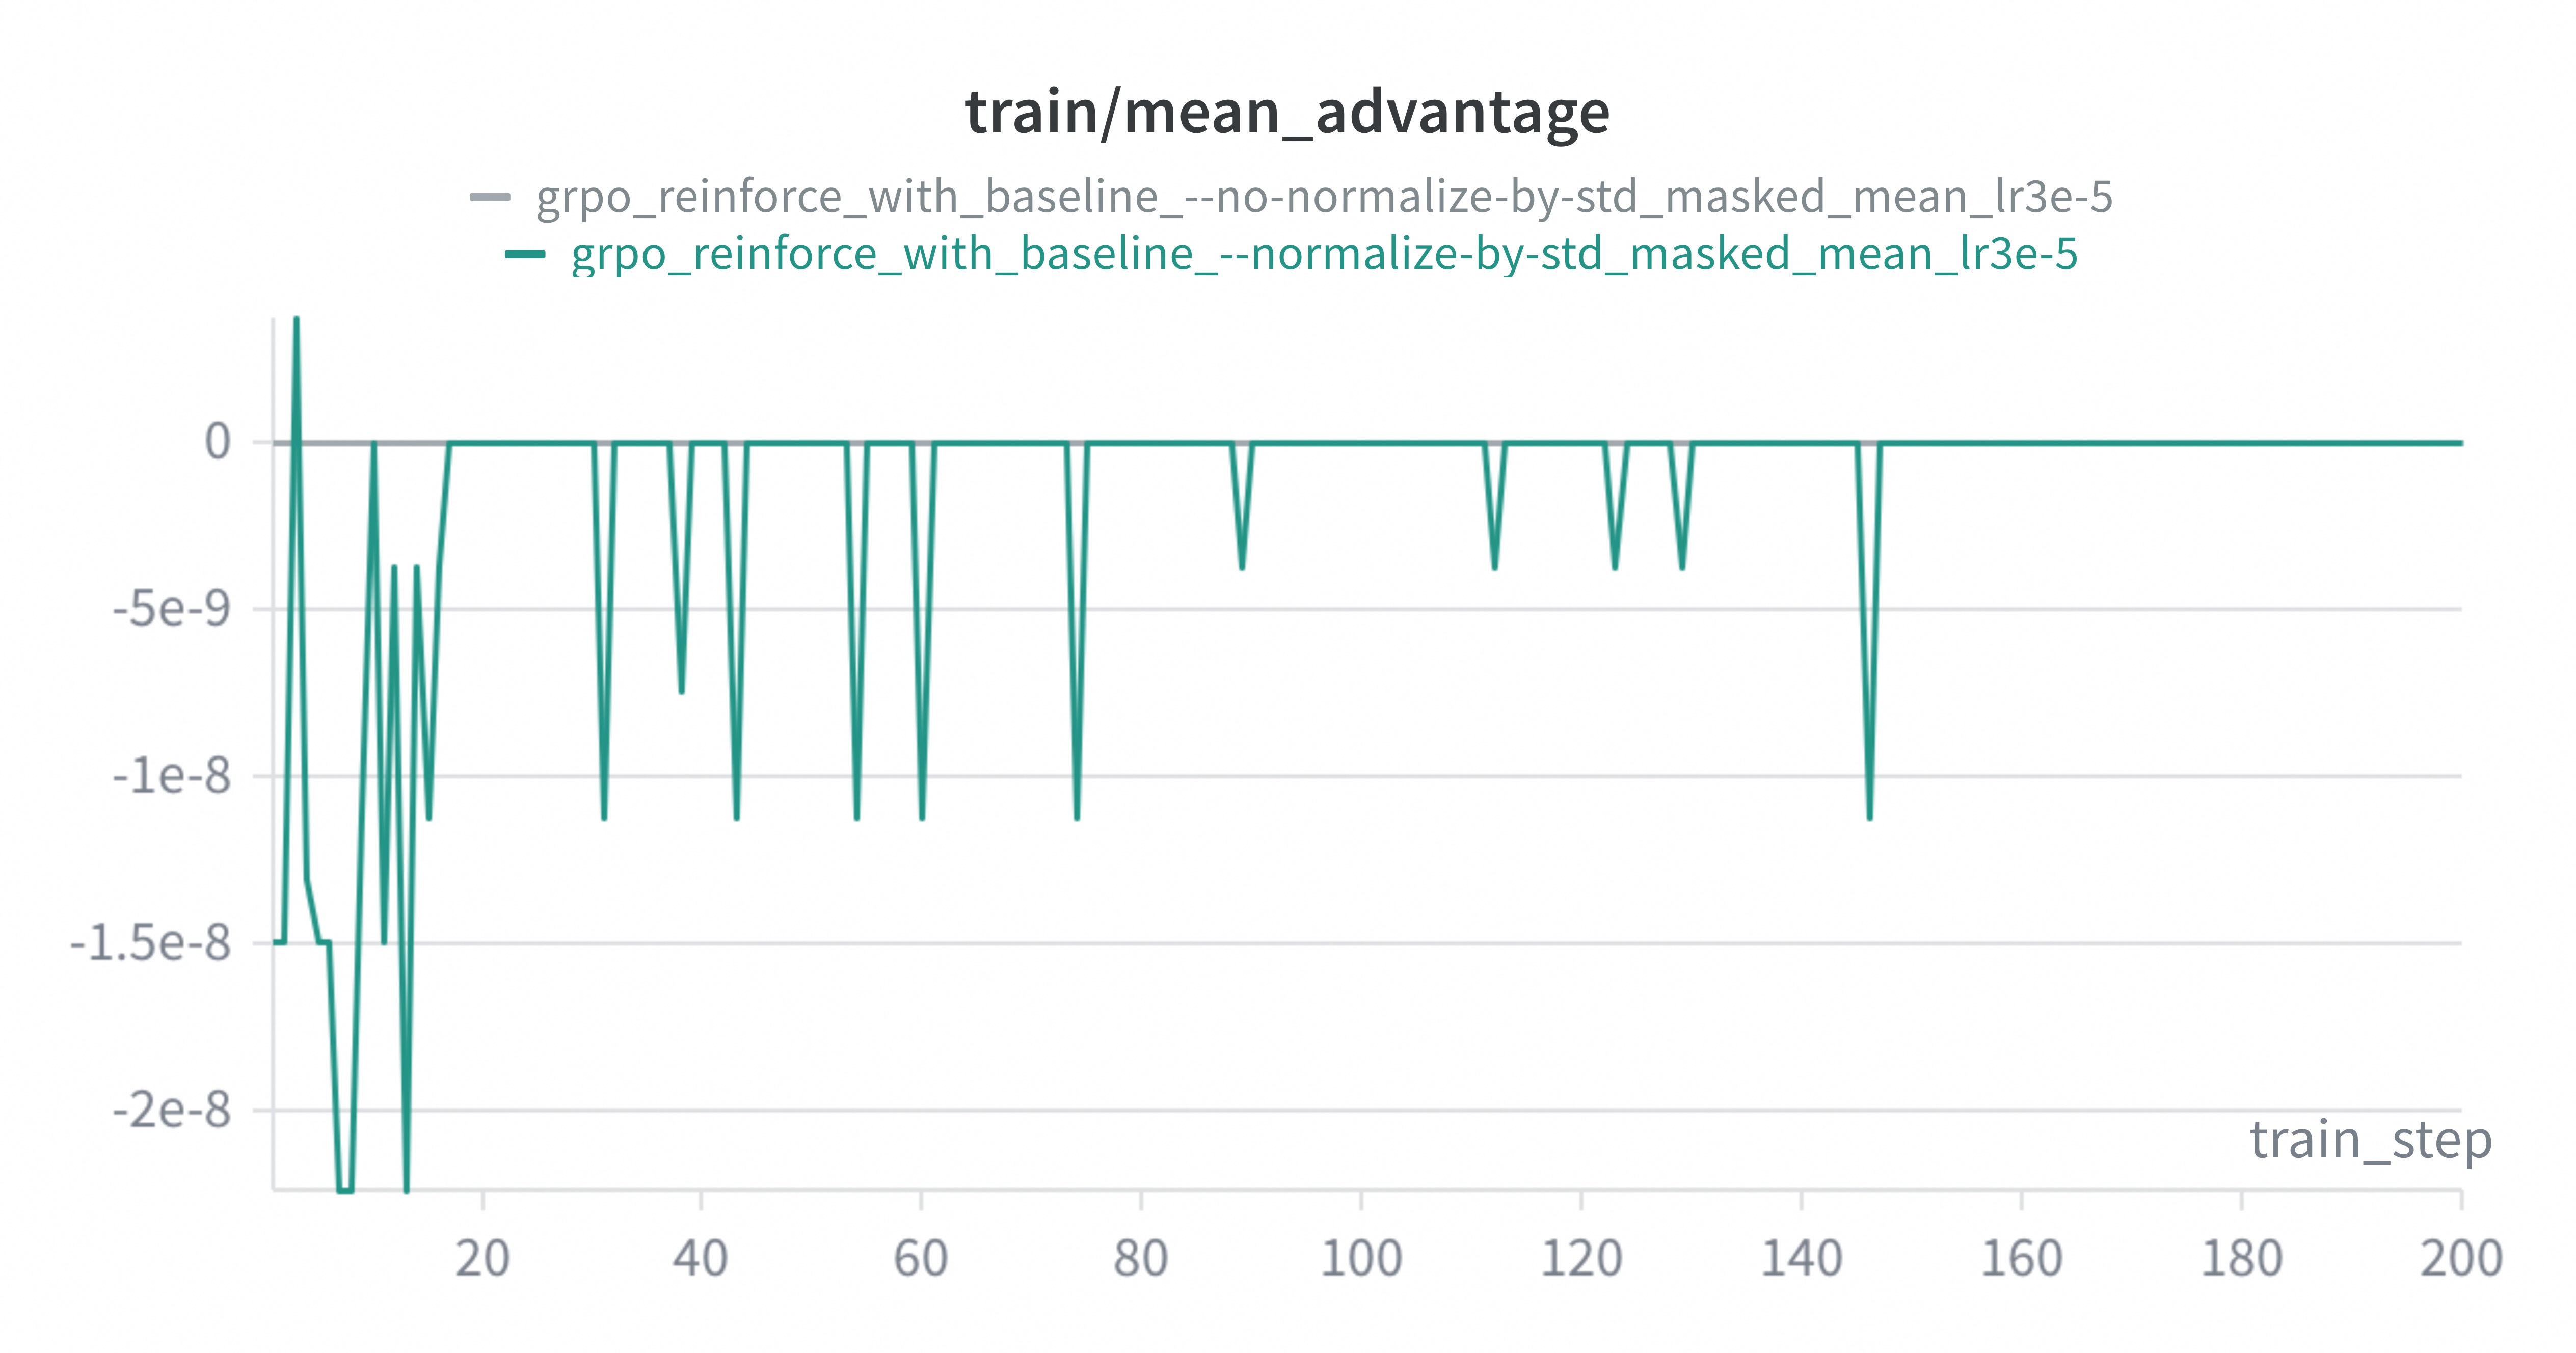
\includegraphics[width=0.9\linewidth]{../charts/grpo_no_std_adv.jpg}
                \end{center}
                We can see that the reward increase for the normalized-by-std and no-normalize-by-std runs are mostly similar. Compared to the normalized-by-std run, the no-normalize-by-std run shows consistently lower gradient norms, while the spike frequency is broadly similar, suggesting slightly more stability for the no-normalize-by-std run. The mean advantage stays at approximately zero throughout the no-normalize run, which is expected from mean-centering without standard-deviation scaling. Despite these optimization-scale differences, the reward curves are largely similar, suggesting comparable task-level performance on Countdown.
            %\item[\textbf{8.1.6}] \textbf{\texttt{grpo\_off\_policy}}
        \end{enumerate}
\end{enumerate}

\end{document}